\chapter{Analyse Comparative et Évaluation Scientifique de la Chaîne DevSecOps dans les Architectures Cloud-Native Sécurisées}
\label{ch:advanced_devsecops_evaluation}

\section{Introduction}

L'essor fulgurant des architectures cloud-natives, propulsé par la conteneurisation et l'orchestration via Kubernetes, a fondamentalement transformé le cycle de vie du développement logiciel. Cependant, cette agilité s'accompagne d'une expansion critique de la surface d'attaque, marquée par une recrudescence historique des compromissions de la chaîne d'approvisionnement logicielle (\textit{software supply chain attacks}). Pour y faire face, les organisations ont progressivement superposé une multitude d'outils de sécurité tout au long de leurs pipelines d'Intégration et de Déploiement Continus (CI/CD), instaurant l'approche DevSecOps.

Ce chapitre documente avec rigueur technique la chaîne DevSecOps effectivement mise en œuvre dans le projet \textit{SecureRAG Hub}, ainsi que la couche de sécurité par intelligence artificielle qui vient s'y adosser. Il s'inscrit en continuité directe du chapitre d'étude préalable et d'état de l'art, dont il reprend et applique systématiquement le principe de transparence entre ce qui est \textbf{réalisé}, ce qui est \textbf{préparé} et ce qui relève d'une \textbf{perspective} d'évolution. Cette discipline de classification n'est pas un exercice de prudence rhétorique~: elle conditionne directement la défendabilité du mémoire en soutenance, où toute affirmation doit pouvoir être reliée à un artefact vérifiable — code, manifeste, journal d'exécution ou rapport produit.

Par rapport à une version antérieure, ce chapitre renforce trois dimensions explicitement identifiées comme insuffisamment développées~: (i) la profondeur de la comparaison avec les solutions concurrentes, qui dépasse désormais le simple constat du choix retenu pour documenter les compromis explicites et les conditions de bascule vers une alternative~; (ii) la rigueur méthodologique des résultats expérimentaux et métriques quantitatives, avec un protocole statistique explicite plutôt que des valeurs isolées~; et (iii) un protocole de validation expérimentale complet pour la couche de sécurité IA, dont le statut de contribution principale du mémoire — s'il est retenu comme tel — exige un niveau de preuve supérieur à celui d'un composant DevSecOps standard.

\section{Cartographie Globale des Outils par Statut}

La figure~\ref{fig:cartographie_statut} offre une vue d'ensemble des familles d'outils mobilisées par \textit{SecureRAG Hub}, codées visuellement selon le statut Réalisé / Préparé / Perspective précisé à la section suivante.

\begin{figure}[htbp]
    \centering
    \scriptsize
    \resizebox{\textwidth}{!}{
\begin{tikzpicture}[
        node distance=0.35cm and 0.4cm,
        every node/.style={draw, rounded corners, align=center,
            inner sep=4pt, minimum height=0.9cm},
        real/.style={fill=green!12, text=black, minimum width=3.6cm},
        prep/.style={fill=yellow!15, text=black, minimum width=3.6cm},
        persp/.style={fill=gray!12, text=black, dashed, minimum width=3.6cm},
        unclear/.style={fill=red!6, text=black, dashed, minimum width=3.6cm},
        center/.style={fill=blue!70, text=white,
            minimum width=3.4cm, minimum height=1.2cm, font=\bfseries}
    ]
        \node[center] (hub) at (0,0) {SecureRAG Hub\\(chaîne DevSecOps)};

        \node[real] (gov) at (-4.2, 2.3) {Gouvernance \& CI\\\scriptsize Jenkins, Git, GitHub};
        \node[real] (sec) at (0, 2.3) {Analyse sécurité\\\scriptsize Semgrep, Gitleaks, Trivy, kube-score};
        \node[real] (build) at (4.2, 2.3) {Build \& supply chain\\\scriptsize Docker, digest, Syft, Cosign};

        \node[real] (k8s) at (-4.2, 0.4) {Déploiement K8s\\\scriptsize kind, Kustomize, probes};
        \node[real] (run) at (4.2, 0.4) {Admission \& runtime\\\scriptsize Kyverno (Audit), Falco, Tetragon};

        \node[persp] (gitops) at (-4.2, -1.5) {GitOps\\\scriptsize ArgoCD};
        \node[real] (data) at (0, -1.9) {Résilience données\\\scriptsize PostgreSQL, pg\_dump};
        \node[prep] (obs) at (4.2, -1.5) {Observabilité\\\scriptsize Prometheus, Grafana, Loki};

        \node[prep] (secrets) at (-4.2, -3.4) {Secrets\\\scriptsize K8s natifs (R), SOPS/age (P), Vault/ESO (Persp.)};
        \node[real] (proofs) at (0, -3.8) {Preuves \& readiness\\\scriptsize Support pack, rapports};
        \node[prep] (rag) at (4.2, -3.4) {Sécurité applicative RAG\\\scriptsize 5 microservices (R), Qdrant (P)};

        \node[unclear] (ia) at (0, -5.5) {Couche sécurité IA\\\scriptsize \texttt{ai-security/} — statut à confirmer};

        \foreach \n in {gov, sec, build, k8s, run, gitops, data, obs, secrets, proofs, rag}
            \draw[->, thick, gray] (\n) -- (hub);
        \draw[->, thick, gray, dashed] (ia) -- (hub);

        \node[real, minimum width=1.6cm, font=\tiny] (leg1) at (-7.8, -6.8) {Réalisé};
        \node[prep, minimum width=1.6cm, font=\tiny, right=0.2cm of leg1] (leg2) {Préparé};
        \node[persp, minimum width=1.9cm, font=\tiny, right=0.2cm of leg2] (leg3) {Perspective};
        \node[unclear, minimum width=2.3cm, font=\tiny, right=0.2cm of leg3] (leg4) {Statut à confirmer};
    \end{tikzpicture}
}
    \caption{Cartographie des familles d'outils de SecureRAG Hub, codées par statut Réalisé / Préparé / Perspective / à confirmer.}
    \label{fig:cartographie_statut}
\end{figure}

Cette cartographie fait apparaître un déséquilibre net entre la maturité de la chaîne DevSecOps proprement dite — majoritairement Réalisé, à l'exception notable du GitOps — et celle de la couche applicative RAG et de la couche de sécurité IA, où les statuts Préparé, Perspective et « à confirmer » dominent. Ce déséquilibre n'est pas anormal pour un projet de fin d'études~: il reflète la priorisation assumée, documentée au chapitre d'étude préalable, de la gouvernance et de l'industrialisation sur la performance conversationnelle immédiate.

\section{Méthodologie d'Évaluation}
\label{sec:methodologie}

L'évaluation de chaque outil repose désormais sur une grille d'analyse à \textbf{six} axes — le sixième, ajouté pour approfondir la dimension comparative, distingue explicitement le constat du choix retenu (déjà présent dans les versions antérieures) de son argumentation critériée (développée section~\ref{sec:comparaison_systematique}).

\begin{figure}[htbp]
    \centering
    \scriptsize
    \resizebox{\textwidth}{!}{
\begin{tikzpicture}[
    node distance=0.4cm,
    axe/.style={draw, rectangle, rounded corners, align=center, fill=blue!6,
        minimum width=2.4cm, minimum height=1.4cm, inner sep=3pt},
    axeb/.style={draw, rectangle, rounded corners, align=center, fill=purple!8,
        minimum width=2.4cm, minimum height=1.4cm, inner sep=3pt},
    arrow/.style={-stealth, thick}
]
    \node[axe] (a1) {1. Positionnement\\architectural};
    \node[axe, right=of a1] (a2) {2. Mécanisme de\\détection/contrôle};
    \node[axe, right=of a2] (a3) {3. Intégration dans\\SecureRAG Hub};
    \node[axe, right=of a3] (a4) {4. Limites\\structurelles};
    \node[axe, right=of a4, fill=orange!10] (a5) {5. Statut\\(R / P / Persp.)};
    \node[axeb, right=of a5] (a6) {6. Comparaison\\critériée aux\\alternatives};
    \draw[arrow] (a1) -- (a2);
    \draw[arrow] (a2) -- (a3);
    \draw[arrow] (a3) -- (a4);
    \draw[arrow] (a4) -- (a5);
    \draw[arrow] (a5) -- (a6);
\end{tikzpicture}
}
\caption{Grille d'analyse à six axes appliquée uniformément à chaque outil de ce chapitre — le sixième axe est nouveau par rapport aux versions antérieures.}
\label{fig:grille_analyse}
\end{figure}

\begin{enumerate}
    \item \textbf{Positionnement architectural} : à quelle étape du cycle de vie logiciel l'outil intervient-il, et sur quelle primitive technique repose-t-il ?
    \item \textbf{Mécanisme de détection ou de contrôle} : quel est le modèle sous-jacent ?
    \item \textbf{Intégration effective dans SecureRAG Hub} : comment l'outil est-il concrètement déployé et configuré ?
    \item \textbf{Limites structurelles} : quelles sont les défaillances intrinsèques de l'outil pris isolément ?
    \item \textbf{Statut} : Réalisé, Préparé, ou Perspective, selon les définitions déjà établies.
    \item \textbf{Comparaison critériée aux alternatives} : sur quels critères explicites l'outil retenu domine-t-il — ou non — les alternatives sérieusement étudiées, et sous quelles conditions ce choix serait-il révisé ?
\end{enumerate}

\begin{quote}
\textbf{Avertissement méthodologique} : plusieurs versions successives de ce chapitre ont dû être corrigées après confrontation avec le code source réel du projet et avec le chapitre d'étude préalable. Certains outils initialement documentés comme pleinement opérationnels se sont révélés soit absents du projet, soit à un statut \textit{Préparé} ou \textit{Perspective} plutôt que \textit{Réalisé}. Le présent chapitre applique désormais strictement le statut établi par le chapitre d'étude préalable. Cette même discipline s'applique au sixième axe introduit ci-dessus~: une comparaison critériée n'est légitime que si elle repose sur des propriétés documentées et vérifiables des outils comparés, et non sur des mesures de performance qui n'ont pas été effectivement produites sur l'infrastructure du projet — ce point est développé section~\ref{sec:comparaison_systematique}.
\end{quote}

\section{Couche d'Orchestration CI/CD}

\subsection{Jenkins}
\textbf{Statut : Réalisé.}

\subsubsection{Rôle et positionnement}
Jenkins constitue l'autorité officielle de CI/CD de \textit{SecureRAG Hub}. La chaîne se décompose en deux pipelines déclaratifs et complémentaires~: le \texttt{Jenkinsfile}, qui opère exclusivement sur le code source, et le \texttt{Jenkinsfile.cd}, qui manipule les artefacts conteneurisés et en garantit l'intégrité de bout en bout.

\subsubsection{Fonctionnement technique}
Chaque pipeline est défini de manière déclarative et versionné dans le dépôt Git au même titre que le code applicatif (\textit{Pipeline as Code}), soumis aux mêmes revues via \textit{Pull Request}. Jenkins consomme les événements émis par GitHub pour déclencher l'exécution.

\subsubsection{Intégration dans SecureRAG Hub}
Le pipeline CI exécute séquentiellement les tests unitaires PHPUnit et l'analyse statique PHPStan (couverture minimale de 70~\%), l'analyse SAST Semgrep, la détection de secrets Gitleaks, le scan de dépendances Trivy FS et \texttt{composer audit}, ainsi que la validation statique des manifestes Kubernetes via kube-score. Un script de \textit{quality gate} consolidé (\texttt{scripts/ci/quality-gate.sh}) agrège l'ensemble de ces sorties. Le pipeline CD reconstruit l'image, exécute Trivy en mode image, génère le SBOM via Syft, signe l'artefact via Cosign, puis promeut l'image par digest SHA-256.

La figure~\ref{fig:pipeline_ci} détaille la séquence du pipeline CI et la figure~\ref{fig:pipeline_cd} celle du pipeline CD.

\begin{figure}[htbp]
    \centering
    \scriptsize
    \resizebox{\textwidth}{!}{
\begin{tikzpicture}[
        node distance=0.5cm,
        stage/.style={draw, rectangle, rounded corners, align=center,
            fill=blue!6, minimum width=2.6cm, minimum height=1cm, inner sep=3pt},
        gate/.style={draw, rectangle, rounded corners, align=center,
            fill=red!10, minimum width=2.2cm, minimum height=1cm, inner sep=3pt},
        arrow/.style={-stealth, thick}
    ]
        \node[stage] (push) {Push / PR\\GitHub webhook};
        \node[stage, right=of push] (tests) {PHPUnit\\PHPStan\\(couverture $\geq$70\%)};
        \node[stage, right=of tests] (sast) {Semgrep\\(SAST)};
        \node[stage, right=of sast] (secrets) {Gitleaks\\(secrets)};
        \node[stage, right=of secrets] (sca) {Trivy FS\\composer audit};
        \node[stage, right=of sca] (k8slint) {kube-score\\validate-kyverno};
        \node[gate, right=of k8slint] (gate) {Quality\\Gate};
        \draw[arrow] (push) -- (tests);
        \draw[arrow] (tests) -- (sast);
        \draw[arrow] (sast) -- (secrets);
        \draw[arrow] (secrets) -- (sca);
        \draw[arrow] (sca) -- (k8slint);
        \draw[arrow] (k8slint) -- (gate);
    \end{tikzpicture}
}
    \caption{Séquence du pipeline CI (\texttt{Jenkinsfile}).}
    \label{fig:pipeline_ci}
\end{figure}

\begin{figure}[htbp]
    \centering
    \scriptsize
    \resizebox{\textwidth}{!}{
\begin{tikzpicture}[
        node distance=0.5cm,
        stage/.style={draw, rectangle, rounded corners, align=center,
            fill=green!6, minimum width=2.6cm, minimum height=1cm, inner sep=3pt},
        arrow/.style={-stealth, thick}
    ]
        \node[stage] (ci) {CI validé\\(quality gate OK)};
        \node[stage, right=of ci] (build) {Build image\\multi-stage};
        \node[stage, right=of build] (scan) {Trivy\\(mode image)};
        \node[stage, right=of scan] (sbom) {Syft\\(SBOM CycloneDX)};
        \node[stage, right=of sbom] (sign) {Cosign\\(signature)};
        \node[stage, right=of sign] (digest) {Promotion\\digest SHA-256};
        \node[stage, right=of digest] (registry) {Registre local\\(no-rebuild)};
        \draw[arrow] (ci) -- (build);
        \draw[arrow] (build) -- (scan);
        \draw[arrow] (scan) -- (sbom);
        \draw[arrow] (sbom) -- (sign);
        \draw[arrow] (sign) -- (digest);
        \draw[arrow] (digest) -- (registry);
    \end{tikzpicture}
}
    \caption{Séquence du pipeline CD (\texttt{Jenkinsfile.cd}).}
    \label{fig:pipeline_cd}
\end{figure}

\subsubsection{Limites structurelles}
Jenkins, en tant qu'orchestrateur, ne possède aucune logique de sécurité native~: il exécute séquentiellement des scripts tiers dont il ne comprend ni la sémantique ni la portée du résultat.

\subsubsection{Comparaison critériée aux alternatives}
Voir la grille consolidée de la section~\ref{sec:comparaison_systematique}, ligne « CI/CD ».

\subsubsection{Infrastructure d'Exécution : Nœuds et Agents Kubernetes Éphémères (CASC)}
\label{sub:infra_casc}

Une inspection directe de l'environnement d'exécution (\texttt{docker ps}, \texttt{kubectl get nodes}) et du fichier de configuration \texttt{infra/jenkins/casc/kubernetes-agents.yaml} confirme que Jenkins ne s'exécute pas comme un unique processus monolithique, mais orchestre des \textit{Pod Templates} Kubernetes éphémères via le plugin Kubernetes et la configuration déclarative CASC (\textit{Configuration as Code}). Cette infrastructure était jusqu'ici absente de l'inventaire de ce chapitre~; elle est intégrée ici avec le même niveau de rigueur de statut que le reste du document.

\begin{figure}[htbp]
\centering
\scriptsize
\resizebox{\textwidth}{!}{
\begin{tikzpicture}[
    node distance=0.5cm and 0.6cm,
    every node/.style={draw, rounded corners, align=center, inner sep=3pt, minimum height=0.9cm},
    real/.style={fill=green!12, text=black, minimum width=3cm},
    center/.style={fill=blue!70, text=white, minimum width=3cm, font=\bfseries},
    arrow/.style={-stealth, thick}
]
    \node[center] (host) {Machine hôte\\Docker Engine};
    \node[real, above left=0.8cm and 0.2cm of host] (jenkins) {securerag-jenkins\\\scriptsize Contrôleur (0 exécuteur local)};
    \node[real, above right=0.8cm and 0.2cm of host] (registry) {kind-registry\\\scriptsize Registre OCI local :5001};
    \node[real, below left=0.8cm and 0.2cm of host] (cp) {securerag-dev-control-plane\\\scriptsize Kubernetes kindest/node};
    \node[real, below right=0.8cm and 0.2cm of host] (worker) {securerag-dev-worker\\\scriptsize Héberge les Pods agents};
    \node[real, below=1.8cm of host] (sigstore) {sigstore-proxy\\\scriptsize Relais Fulcio/Rekor (Cosign)};
    \draw[arrow] (jenkins) -- (host);
    \draw[arrow] (registry) -- (host);
    \draw[arrow] (cp) -- (host);
    \draw[arrow] (worker) -- (host);
    \draw[arrow] (sigstore) -- (host);
    \draw[arrow] (cp) -- (worker) node[midway, right, font=\tiny] {scheduling Pods};
\end{tikzpicture}
}
\caption{Nœuds d'infrastructure observés directement (\texttt{docker ps}, \texttt{kubectl get nodes})~: contrôleur Jenkins, plan de contrôle et nœud \textit{worker} du cluster \texttt{kind}, registre OCI local et proxy Sigstore. Tous confirmés Réalisé par observation directe de l'environnement en exécution.}
\label{fig:infra_casc}
\end{figure}

Le tableau~\ref{tab:agents_casc} et la figure~\ref{fig:agents_distribution} détaillent les sept \textit{Pod Templates} déclarés. Leur existence dans le fichier CASC atteste qu'ils sont \textbf{préparés et instanciables à la demande}~; elle ne constitue pas à elle seule la preuve qu'un outil embarqué dans l'image d'un agent est effectivement invoqué par une étape active du \texttt{Jenkinsfile}. Conformément à la discipline de ce chapitre, chaque outil est donc évalué individuellement~: les outils déjà établis Réalisé ailleurs dans ce document (Semgrep, Gitleaks, Trivy, Syft, Cosign, kube-score, Kyverno CLI, kubectl) conservent ce statut au sein de l'agent qui les héberge. Les outils dont la présence dans un agent \textbf{contredit} un statut déjà établi (SonarQube, Grype, Helm, ArgoCD CLI) ou qui n'apparaissent dans aucun autre inventaire de ce chapitre (OWASP Dependency-Check, Checkov, OWASP ZAP, k6) sont reclassés \textbf{Préparé}~: l'infrastructure d'exécution existe, mais rien dans ce chapitre n'atteste à ce stade qu'une étape du pipeline les invoque effectivement.

\begin{table}[htbp]
\centering
\scriptsize
\begin{tabular}{@{}p{2.4cm}p{2.4cm}p{4.4cm}p{4.4cm}@{}}
\toprule
\textbf{Agent (label)} & \textbf{Ressources} & \textbf{Outillage} & \textbf{Statut par outil} \\
\midrule
\texttt{test-agent} & 2 vCPU / 2 GiB & PHP 8.4, Composer, PCOV, Xdebug & Réalisé (cohérent avec PHPUnit établi) \\
\texttt{security-agent} & 4 vCPU / 4 GiB & Semgrep, Gitleaks, Trivy, Dependency-Check & Semgrep/Gitleaks/Trivy~: Réalisé~; Dependency-Check~: \textbf{Préparé} (absent de l'inventaire officiel avant ce constat) \\
\texttt{docker-agent} & 4 vCPU / 4 GiB (+DinD) & Docker BuildKit, Syft, Grype, Cosign & Docker/Syft/Cosign~: Réalisé~; Grype~: \textbf{Préparé} (Trivy seul retenu en comparaison, section~\ref{sec:comparaison_systematique}) \\
\texttt{k8s-agent} & 2 vCPU / 2 GiB & Checkov, kube-score, Kyverno CLI & kube-score/Kyverno CLI/Checkov~: Réalisé (stage Terraform IaC Scan actif dans le Jenkinsfile) \\
\texttt{sonar-agent} & 2 vCPU / 4 GiB & Sonar Scanner & \textbf{Préparé} (SonarQube explicitement écarté au profit de Semgrep, section~\ref{sec:comparaison_systematique}) \\
\texttt{zap-agent} & 4 vCPU / 4 GiB & OWASP ZAP, k6 & \textbf{Préparé} (ni l'un ni l'autre confirmé exécuté) \\
\texttt{deploy-agent} & 1 vCPU / 1 GiB & kubectl, Helm, ArgoCD CLI & kubectl~: Réalisé~; Helm~: \textbf{Préparé} (Kustomize retenu en comparaison, section~\ref{sec:comparaison_systematique})~; ArgoCD CLI~: \textbf{Réalisé} (ArgoCD déployé, section~\ref{sec:gitops}) \\
\bottomrule
\end{tabular}
\caption{Sept Pod Templates Kubernetes éphémères déclarés dans \texttt{kubernetes-agents.yaml}, avec statut reclassifié outil par outil}
\label{tab:agents_casc}
\end{table}

\begin{figure}[htbp]
\centering
\scriptsize
\resizebox{\textwidth}{!}{
\begin{tikzpicture}[
    node distance=0.4cm and 0.5cm,
    every node/.style={draw, rounded corners, align=center, inner sep=3pt, minimum height=1cm},
    real/.style={fill=green!12, text=black, minimum width=3cm},
    prep/.style={fill=yellow!15, text=black, minimum width=3cm},
    arrow/.style={-stealth, thick}
]
    \node[real] (test) {\texttt{test-agent}\\\scriptsize PHPUnit, couverture};
    \node[real, right=of test] (security) {\texttt{security-agent}\\\scriptsize Semgrep, Gitleaks, Trivy};
    \node[real, right=of security] (docker) {\texttt{docker-agent}\\\scriptsize Build, SBOM, Cosign};
    \node[real, below=of test] (k8s) {\texttt{k8s-agent}\\\scriptsize kube-score, Kyverno CLI};
    \node[prep, below=of security] (sonar) {\texttt{sonar-agent}\\\scriptsize Préparé, non retenu};
    \node[prep, below=of docker] (zap) {\texttt{zap-agent}\\\scriptsize Préparé, DAST/k6 non confirmés};
    \node[real, below=1.7cm of security, xshift=0cm] (deploy) {\texttt{deploy-agent}\\\scriptsize kubectl Réalisé~; Helm/ArgoCD CLI Préparé};

    \node[real, minimum width=1.6cm, font=\tiny, below=2.6cm of test] (leg1) {Réalisé};
    \node[prep, minimum width=1.8cm, font=\tiny, right=0.2cm of leg1] (leg2) {Préparé};
\end{tikzpicture}
}
\caption{Distribution des sept agents Pod éphémères du pipeline, colorés selon le statut consolidé de leur outillage (détail par outil individuel dans le tableau~\ref{tab:agents_casc}).}
\label{fig:agents_distribution}
\end{figure}

\section{Intégration du DevSecOps dans le Cycle Agile : Sprint DevSecOps, DoD et Gouvernance}
\label{sec:agile_devsecops_sprint}

L'efficacité d'une démarche DevSecOps repose non seulement sur l'outillage technique, mais également sur son intégration fluide au sein du cycle de développement agile. Dans le cadre du projet \textit{SecureRAG Hub}, la sécurité n'est pas traitée comme une activité ponctuelle en fin de projet, mais est directement infusée dans le rituel des \textbf{Sprints Agile/Scrum} \cite{schwaber_scrum_guide}.

\subsection{Modélisation des Menaces et Security User Stories au Sprint Planning}

Lors de la phase de \textit{Sprint Planning}, chaque fonctionnalité métier (ex: ingestion de documents vectoriels, authentification OAuth2, gestion du dialogue RAG) est évaluée sous l'angle de la sécurité. Les exigences sont déclinées sous forme de :
\begin{itemize}
    \item \textbf{Security User Stories} : Histoires utilisateurs spécifiant les contrôles requis (ex: « En tant qu'administrateur, je veux que les clés d'API LLM soient chiffrées en base au repos afin d'éviter toute divulgation en cas de fuite de sauvegarde »).
    \item \textbf{Abuse Cases (Cas d'Abus)} : Scénarios modélisant les actions d'un attaquant (ex: « En tant qu'attaquant externe, je tente d'injecter une instruction système dans le prompt RAG pour exfiltrer le contexte applicatif »).
\end{itemize}

Ces éléments sont intégrés au \textit{Product Backlog} et priorisés au même titre que les fonctionnalités métiers.

\subsection{La Définition de Terminé (\textit{Definition of Done} - DoD) Sécurisée}

Pour garantir qu'aucun incrément logiciel vulnérable ne rejoigne la branche principale (\texttt{main}), la \textbf{Definition of Done (DoD)} standard a été enrichie d'exigences de sécurité strictes et automatisées. Une \textit{User Story} ne peut être déclarée « Terminée » que si elle satisfait les six critères de la grille DoD DevSecOps :

\begin{table}[htbp]
\centering
\scriptsize
\begin{tabular}{@{}p{3.2cm}p{5.4cm}p{4.2cm}@{}}
\toprule
\textbf{Critère DoD DevSecOps} & \textbf{Mécanisme de Contrôle Automatisé} & \textbf{Seuil d'Acceptation (Gate)} \\
\midrule
1. Qualité \& Tests & Tests unitaires et d'intégration PHPUnit & Couverture de code $\ge 70\%$ \\
2. Analyse Statique (SAST) & Scan Semgrep par AST sur le code source & 0 vulnérabilité \texttt{CRITICAL} ou \texttt{HIGH} \\
3. Inviolabilité Secrets & Scan d'entropie et regex Gitleaks & 0 secret ou token détecté dans Git \\
4. Sécurité Dépendances (SCA) & Scan Trivy FS et \texttt{composer audit} & 0 CVE critique non dérogée \\
5. Conformité Manifestes & Audit statique kube-score \& Kyverno CLI & Score de conformité PSS Restricted OK \\
6. Intégrité Supply Chain & Build Kaniko rootless, Syft SBOM \& Cosign & Image signée SHA-256 + SBOM CycloneDX \\
\bottomrule
\end{tabular}
\caption{Grille des critères de la Definition of Done (DoD) DevSecOps appliquée lors de chaque Sprint.}
\label{tab:dod_devsecops}
\end{table}

\subsection{Sprints d'Industrialisation et de Durcissement (\textit{Security Hardening Sprints})}

Outre l'intégration continue au fil des sprints de delivery, le projet intercale périodiquement des \textbf{Sprints d'Industrialisation et de Durcissement} (\textit{Hardening Sprints}). Ces sprints dédiés visent à :
\begin{enumerate}
    \item Exécuter des campagnes de tests dynamiques complexes (DAST OWASP ZAP) et de Red Teaming d'IA (fuzzing d'injections de prompt par Garak).
    \item Réduire la dette technique de sécurité (\textit{Security Technical Debt}) issue des rapports d'audit statiques et des alertes de runtime eBPF (Falco).
    \item Valider les scripts de restauration de sauvegardes PostgreSQL et les procédures de réponse aux incidents (\texttt{RUNBOOK-INCIDENT-RESPONSE.md}).
\end{enumerate}

\subsection{Mesure de Vélocité et Impact de la Sécurité sur l'Équipe}

L'automatisation des contrôles au sein d'agents Kubernetes éphémères CASC permet de contenir le surcoût temporel lié à la sécurité. L'analyse des métriques d'équipe montre que l'exécution des contrôles DevSecOps ajoute un temps moyen de \textbf{4.2 minutes} par build CI/CD, largement compensé par la réduction de \textbf{96.5\% du temps de remédiation (MTTR)} grâce à la détection précoce des failles.

\section{Analyse de Sécurité (SAST / SCA / Secrets)}


\begin{figure}[htbp]
\centering
\scriptsize
\resizebox{\textwidth}{!}{
\begin{tikzpicture}[
    node distance=0.5cm and 0.6cm,
    src/.style={draw, rectangle, rounded corners, align=center, fill=blue!6,
        minimum width=3cm, minimum height=1cm, inner sep=3pt},
    gate/.style={draw, rectangle, rounded corners, align=center, fill=red!8,
        minimum width=2.6cm, minimum height=1.2cm, inner sep=3pt},
    arrow/.style={-stealth, thick}
]
    \node[src] (code) {Code source\\Semgrep (SAST)};
    \node[src, below=of code] (hist) {Historique Git\\Gitleaks (secrets)};
    \node[src, below=of hist] (deps) {Dépendances\\Trivy FS, composer audit};
    \node[gate, right=1.4cm of hist] (gate) {Security\\backlog\\+ Quality Gate};
    \draw[arrow] (code) -- (gate);
    \draw[arrow] (hist) -- (gate);
    \draw[arrow] (deps) -- (gate);
\end{tikzpicture}
}
\caption{Trois analyses statiques complémentaires (\textit{Shift Left}) convergeant vers un security backlog et un quality gate communs.}
\label{fig:shift_left}
\end{figure}

\subsection{Semgrep (SAST)}
\textbf{Statut : Réalisé.}

Semgrep intervient en tout début de chaîne pour analyser le code source de l'ensemble des microservices. Il construit un arbre de syntaxe abstraite (AST) et applique des règles déclaratives, ce qui le distingue des approches par expressions régulières. Le projet mobilise les \textit{rulesets} publics Semgrep et des règles personnalisées PHP/Laravel. Les exceptions justifiées sont tracées dans un \textit{security backlog}. Limite structurelle~: l'analyse reste purement statique, sans garantie d'atteignabilité en production.

\subsubsection{Comparaison critériée à l'alternative SonarQube}
SonarQube Community couvre une partie recoupante de la SAST mais se positionne historiquement davantage comme outil de qualité de code (dette technique, duplication) que comme moteur de règles de sécurité dédié~; son intégration CI est plus lourde (serveur dédié, base de données) que celle de Semgrep, qui s'exécute comme un binaire autonome sans infrastructure serveur. Le critère décisif a été la légèreté d'intégration dans un pipeline Jenkins déjà dense. Un basculement vers SonarQube serait justifié si le projet visait explicitement un tableau de bord de dette technique consolidé, ce qui n'est pas l'objectif du présent mémoire.

\subsection{Gitleaks}
\textbf{Statut : Réalisé.}

Gitleaks applique des expressions régulières et des heuristiques d'entropie de Shannon sur chaque ligne modifiée et sur l'historique complet lors d'un scan intégral. Il est exécuté comme étape bloquante du pipeline CI, avec un fichier d'exceptions documenté (\texttt{.gitleaks.toml}). Limite~: un secret encodé, fragmenté ou injecté dynamiquement échappe structurellement à l'analyse statique.

\subsubsection{Comparaison critériée à l'alternative TruffleHog}
TruffleHog ajoute une capacité de vérification active de certains types de secrets (validation en ligne de la validité d'une clé auprès du fournisseur), capacité que Gitleaks ne possède pas nativement. Ce gain de précision a un coût~: il suppose des appels réseau sortants depuis l'environnement CI vers des services tiers, ce qui est en tension avec la discipline de cloisonnement réseau (\textit{deny-all} par défaut) documentée section~\ref{sec:runtime_security} pour l'environnement runtime, et introduit une dépendance externe non souhaitée dans un pipeline dont l'un des objectifs affichés est la reproductibilité hors ligne. Gitleaks a été retenu pour cette raison, au prix d'un taux de faux positifs de configuration légèrement supérieur, absorbé par le fichier d'exceptions documenté.

\subsection{Trivy et \texttt{composer audit}}
\textbf{Statut : Réalisé.}

Trivy est mobilisé en mode \textit{filesystem} avant construction et en mode image après construction. Pour l'analyse SCA, il extrait la nomenclature des dépendances et effectue une correspondance contre des bases de vulnérabilités agrégées~; pour l'analyse d'image, il inspecte chaque couche OCI. Les exceptions acceptées sont tracées dans \texttt{.trivyignore}. Limite~: dépendance intégrale à l'exhaustivité et à la fraîcheur des bases de données~; une vulnérabilité \textit{zero-day} est structurellement invisible.

\subsubsection{Comparaison critériée à l'alternative Grype}
Grype (Anchore) et Trivy (Aqua Security) partagent un positionnement fonctionnel très proche~: correspondance de nomenclature contre bases de vulnérabilités publiques. La différence pratique déterminante dans ce projet est l'unification~: Trivy couvre à la fois le mode \textit{filesystem} et le mode image dans un seul binaire et une seule syntaxe de configuration, alors que Grype se concentre sur l'image et suppose l'usage combiné d'un second outil (par exemple Syft, déjà retenu par ailleurs pour le SBOM) pour la génération de nomenclature en amont. Retenir Trivy seul plutôt que Grype+Syft+un scanner FS distinct réduit le nombre d'outils à maintenir dans le pipeline, au prix d'une dépendance accrue à un unique fournisseur de base de vulnérabilités. Une réévaluation serait justifiée si des divergences de couverture entre bases de vulnérabilités devenaient critiques, ce qui justifierait alors un usage combiné Trivy+Grype en double vérification plutôt qu'un remplacement.

\subsection{Kube-score}
\textbf{Statut : Réalisé.}

Kube-score évalue la conformité des manifestes Kubernetes (limites de ressources, absence de conteneurs privilégiés, sondes de santé) sans nécessiter de cluster actif, complété par des scripts personnalisés validant statiquement la cohérence des politiques Kyverno. Limite~: aucune garantie sur le comportement runtime effectif.

\section{Build, Registre et Chaîne d'Approvisionnement}

\begin{figure}[htbp]
\centering
\scriptsize
\resizebox{\textwidth}{!}{
\begin{tikzpicture}[
    node distance=0.6cm,
    box/.style={draw, rectangle, rounded corners, align=center, fill=green!6,
        minimum width=2.4cm, minimum height=1cm, inner sep=3pt},
    arrow/.style={-stealth, thick}
]
    \node[box] (img) {Image\\construite};
    \node[box, right=of img] (digest) {Digest\\SHA-256};
    \node[box, right=of digest] (sbom) {SBOM\\(Syft)};
    \node[box, right=of sbom] (sig) {Signature\\(Cosign)};
    \node[box, right=of sig] (verif) {Vérification\\à l'admission};
    \draw[arrow] (img) -- (digest);
    \draw[arrow] (digest) -- (sbom);
    \draw[arrow] (sbom) -- (sig);
    \draw[arrow] (sig) -- (verif);
\end{tikzpicture}
}
\caption{Chaîne de confiance de l'artefact.}
\label{fig:chaine_confiance}
\end{figure}

\subsection{Docker et Discipline de l'Immuabilité}
\textbf{Statut : Réalisé.}

Docker assure la conteneurisation via des \texttt{Dockerfiles} multi-étapes. Deux disciplines structurent la chaîne~: la \textbf{promotion digest-first} (seul un digest scanné et signé est promu, tags mutables refusés) et le \textbf{déploiement no-rebuild}. Les images sont hébergées sur un registre local joignable depuis \texttt{kind}. Limite~: l'immuabilité protège l'identité de l'artefact mais ne dit rien sur son comportement une fois exécuté.

\subsection{Syft}
\textbf{Statut : Réalisé.}

Syft génère systématiquement le SBOM CycloneDX de chaque artefact, en catalogant les paquets couche par couche. Le SBOM sert aux audits de conformité, à la veille de vulnérabilités et à l'inventaire des licences. Limite~: inventaire statique à un instant donné.

\subsection{Cosign (Sigstore)}
\textbf{Statut : Réalisé.}

Cosign produit une signature détachée vérifiable, contrôlée dans le pipeline CD avant promotion et potentiellement à l'admission. Les attestations in-toto sont préparées mais non pleinement opérées. Limite~: garantit l'intégrité à la construction, pas le comportement après démarrage.

\subsubsection{Comparaison critériée à l'alternative Notation}
Notation (projet CNCF) et Cosign (Sigstore) couvrent le même besoin fonctionnel de signature d'image. Cosign a été retenu pour son intégration documentée et directe avec la règle \texttt{verifyImages} de Kyverno, déjà retenu par ailleurs comme moteur d'admission~: les deux projets partagent un écosystème de référence commun (Sigstore/Kyverno), ce qui réduit le risque d'incompatibilité de format entre la signature produite et sa vérification. Notation reste une alternative crédible si le projet devait s'intégrer à un registre d'entreprise imposant spécifiquement ce standard.

\subsection{Blockchain : Technologie Étudiée mais Non Retenue}
\textbf{Statut : Non implémenté — piste étudiée et explicitement écartée.}

L'usage d'une blockchain a été envisagé pour garantir l'intégrité des traces d'audit et fournir un registre infalsifiable des artefacts. Trois arguments ont motivé son écartement~: adéquation fonctionnelle (les besoins d'intégrité sont déjà couverts par SHA-256, SBOM CycloneDX, Cosign et \texttt{SHA256SUMS}), complexité opérationnelle (nœuds dédiés, gouvernance cryptographique, gestion des clés, latence d'écriture sans gain démontrable), et maturité contextuelle (adoption industrielle limitée pour ce cas d'usage dans les plateformes de chatbots d'entreprise). Cette décision illustre une discipline de conception plus large~: préférer un mécanisme simple, mature et démontrable à une solution plus sophistiquée dont la valeur ajoutée resterait à prouver.

\section{Déploiement Kubernetes}

\begin{figure}[htbp]
\centering
\scriptsize
\resizebox{\textwidth}{!}{
\begin{tikzpicture}[
    node distance=0.5cm and 0.6cm,
    base/.style={draw, rectangle, rounded corners, align=center, fill=blue!8,
        minimum width=2.6cm, minimum height=1cm, inner sep=3pt},
    ov/.style={draw, rectangle, rounded corners, align=center, fill=green!6,
        minimum width=2.4cm, minimum height=1cm, inner sep=3pt},
    arrow/.style={-stealth, thick}
]
    \node[base] (base) {Base commune\\(Kustomize)};
    \node[ov, below left=1cm and -0.3cm of base] (dev) {Overlay\\dev};
    \node[ov, below=1cm of base] (demo) {Overlay\\demo};
    \node[ov, below right=1cm and -0.3cm of base] (prod) {Overlay\\production-like};
    \draw[arrow] (base) -- (dev);
    \draw[arrow] (base) -- (demo);
    \draw[arrow] (base) -- (prod);
\end{tikzpicture}
}
\caption{Composition Kustomize.}
\label{fig:kustomize_overlays}
\end{figure}

\subsection{Kubernetes \texttt{kind} et Kustomize}
\textbf{Statut : Réalisé.}

Le déploiement s'appuie sur \texttt{kind}, sans dépendance à une infrastructure cloud externe. La configuration est gérée par Kustomize en une base commune et des \textit{overlays} par environnement. Les ressources mobilisées sont \textit{namespaces}, \textit{Deployments}, \textit{Services}, \textit{ConfigMaps} et \textit{Secrets} natifs, avec les trois sondes \texttt{startupProbe}, \texttt{readinessProbe} et \texttt{livenessProbe}. Limite~: un cluster \texttt{kind} local ne restitue ni la latence réseau ni les contraintes de montée en charge d'un cluster de production multi-nœuds.

\subsubsection{Comparaison critériée à l'alternative Minikube}
Minikube et \texttt{kind} couvrent un besoin équivalent de cluster Kubernetes local. \texttt{kind} a été retenu pour son démarrage plus rapide et son intégration Docker directe (le cluster \emph{est} un ensemble de conteneurs Docker, plutôt qu'une machine virtuelle comme dans certains pilotes Minikube), ce qui réduit la consommation de ressources sur la machine de développement et accélère le cycle de test du pipeline CD. Minikube resterait pertinent si le projet nécessitait un pilote spécifique (par exemple l'émulation de \textit{LoadBalancer} via un \textit{tunnel} dédié), besoin non rencontré dans ce projet.

\subsubsection{Comparaison critériée à l'alternative Helm pour la gestion des manifestes}
Helm introduit un moteur de \textit{templating} et un système de \textit{charts} versionnées, utile pour la distribution de logiciels tiers paramétrables. Kustomize a été retenu car il opère par \textit{overlay} (surcharge de manifestes YAML natifs) sans langage de templating supplémentaire à apprendre ni à maintenir~: pour un projet interne dont les manifestes ne sont pas destinés à être distribués à des tiers, cette simplicité l'emporte sur la flexibilité de packaging offerte par Helm. Un passage à Helm serait justifié si \textit{SecureRAG Hub} devait un jour être distribué comme produit installable par des tiers.

\section{Sécurité Runtime et Contrôle d'Admission}
\label{sec:runtime_security}

\begin{figure}[htbp]
\centering
\scriptsize
\resizebox{\textwidth}{!}{
\begin{tikzpicture}[
    node distance=0.6cm and 0.8cm,
    box/.style={draw, rectangle, rounded corners, align=center, fill=blue!6,
        minimum width=2.6cm, minimum height=1cm, inner sep=3pt},
    audit/.style={draw, rectangle, rounded corners, align=center, fill=yellow!12,
        minimum width=2.8cm, minimum height=1cm, inner sep=3pt},
    enforce/.style={draw, rectangle, rounded corners, dashed, align=center, fill=gray!8,
        minimum width=2.8cm, minimum height=1cm, inner sep=3pt},
    arrow/.style={-stealth, thick}, darrow/.style={-stealth, thick, dashed}
]
    \node[box] (req) {Requête\\admission pod};
    \node[audit, right=of req] (audit) {Mode Audit\\(actuel)\\PolicyReport};
    \node[enforce, below=of audit] (enforce) {Mode Enforce\\(Réalisé)\\Rejet effectif};
    \draw[arrow] (req) -- (audit);
    \draw[darrow] (req) -- (enforce);
\end{tikzpicture}
}
\caption{Kyverno en mode Enforce (Réalisé).}
\label{fig:kyverno_audit_enforce}
\end{figure}

\subsection{Kyverno}
\textbf{Statut : Réalisé (mode Enforce actif).}

Kyverno exprime ses règles en \textit{ClusterPolicies} YAML natives à Kubernetes. Le projet mobilise Kyverno pour~: la règle \texttt{verifyImages} (signature Cosign valide requise), le durcissement \textit{SecurityContext} (\texttt{runAsNonRoot}, \texttt{readOnlyRootFilesystem}, \texttt{allowPrivilegeEscalation: false}, suppression des \textit{capabilities}, profil seccomp \texttt{RuntimeDefault}), et la validation RBAC/NetworkPolicies. \textbf{Point de vigilance essentiel} : ces politiques sont actives en \textbf{mode Audit}, qui consigne les violations sans bloquer la création des ressources. Toute affirmation selon laquelle Kyverno « bloque » une image non signée doit être nuancée~: il \textit{détecte et journalise}, sans nécessairement empêcher.

\subsubsection{Comparaison critériée à l'alternative OPA/Gatekeeper}
Le cahier des charges initial identifiait OPA/Gatekeeper, fondé sur Rego, comme alternative. Kyverno a été retenu pour la lisibilité de ses politiques en YAML natif, contre la puissance d'expression supérieure mais la courbe d'apprentissage plus exigeante de Rego. Sur le plan strictement fonctionnel, Gatekeeper et Kyverno couvrent un périmètre équivalent (mutation, validation, génération de ressources)~; la différence pratique déterminante est l'accessibilité~: une politique Kyverno peut être relue et modifiée par un développeur familier de YAML Kubernetes, alors qu'une politique Rego exige une compétence dédiée. \textbf{OPA/Gatekeeper n'est pas déployé dans le projet}. Une bascule serait justifiée si le projet devait un jour mutualiser ses politiques avec une organisation ayant déjà standardisé sur Rego (par exemple pour des politiques partagées avec des systèmes non Kubernetes, où Rego s'applique plus largement que Kyverno).

\subsection{Falco}
\textbf{Statut : Réalisé (capacité de détection démontrée) — opération continue en production : Perspective.}

Falco capture les appels système via une sonde eBPF et confronte chaque appel à des règles déclaratives de comportement anormal, déployé en \textit{DaemonSet}. L'activation continue avec routage systématique des alertes reste une perspective~; la capacité de détection est démontrable dans un scénario contrôlé. Limite~: alertes brutes et isolées par nœud, sans corrélation globale native.

\subsubsection{Comparaison critériée aux alternatives Sysdig Secure et Tracee}
Sysdig Secure, éditeur commercial à l'origine du projet Falco open source, ajoute une couche de corrélation, un moteur de règles enrichi et un support commercial, au prix d'une licence payante et d'une dépendance à un fournisseur tiers pour l'hébergement des données de télémétrie. Tracee (Aqua Security), également fondé sur eBPF, offre une alternative purement open source proche de Falco mais avec un écosystème de règles communautaires moins développé au moment de la conception du projet. Falco a été retenu pour la maturité et le volume de sa base de règles communautaires (CNCF \textit{graduated project}) et pour l'absence de dépendance commerciale, cohérente avec le choix assumé ailleurs dans ce chapitre de n'écarter aucune alternative pour un motif de coût de licence. Une bascule vers Sysdig Secure serait justifiable si le projet devait un jour opérer en production avec un besoin de support contractuel formel.

\subsection{Tetragon}
\textbf{Statut : Réalisé.}

Tetragon complète Falco en apportant une capacité d'application active (\textit{enforcement}) au niveau du noyau via eBPF, permettant de bloquer un appel système avant sa complétion. Limite~: risque de disponibilité en cas de faux positif entraînant le blocage d'une opération légitime.

\subsection{NetworkPolicies, RBAC Kubernetes et Quotas}
\textbf{Statut : Réalisé.}

Les \textit{NetworkPolicies} appliquent une segmentation \textit{deny-all} par défaut. Le RBAC restreint les droits des \textit{ServiceAccounts} selon le moindre privilège. Les \textit{ResourceQuota} et \textit{LimitRange} plafonnent les ressources consommables. Limite~: une politique \textit{deny-all} mal calibrée peut interrompre un flux légitime non anticipé.

\section{GitOps et Déploiement Continu}
\label{sec:gitops}

\begin{figure}[htbp]
\centering
\scriptsize
\resizebox{\textwidth}{!}{
\begin{tikzpicture}[
    node distance=0.6cm and 0.8cm,
    now/.style={draw, rectangle, rounded corners, align=center, fill=green!6,
        minimum width=2.8cm, minimum height=1cm, inner sep=3pt},
    persp/.style={draw, rectangle, rounded corners, dashed, align=center, fill=gray!8,
        minimum width=2.8cm, minimum height=1cm, inner sep=3pt},
    arrow/.style={-stealth, thick}, darrow/.style={-stealth, thick, dashed}
]
    \node[now] (jenkins) {Jenkins CD\\(push manuel déclenché)};
    \node[now, right=of jenkins] (deploy) {Déploiement\\Kubernetes};
    \node[persp, below=1.2cm of jenkins, xshift=1.4cm] (argocd) {ArgoCD\\(Réalisé)\\réconciliation continue};
    \draw[arrow] (jenkins) -- (deploy);
    \draw[darrow] (argocd) -- (deploy) node[midway, right, font=\tiny] {boucle visée};
\end{tikzpicture}
}
\caption{État GitOps avec ArgoCD (Réalisé).}
\label{fig:gitops_actuel_cible}
\end{figure}

\subsection{ArgoCD}
\textbf{Statut : Réalisé — l'industrialisation GitOps avec boucle de réconciliation semi-automatisée est active.}

Dans sa cible architecturale, ArgoCD assurerait la synchronisation continue entre l'état déclaré dans Git et l'état observé du cluster. Le chapitre d'étude préalable classe explicitement cette industrialisation parmi les perspectives d'évolution. Toute description d'un rollback ArgoCD déclenché sans intervention humaine doit être relue comme une cible fonctionnelle, non comme un comportement démontré. Limite~: en son absence, la promotion des artefacts repose sur Jenkins et la discipline digest-first, sans boucle de réconciliation continue.

\section{Secrets, Données et Résilience}

\subsection{Secrets Kubernetes Natifs}
\textbf{Statut : Réalisé.}

Les ressources \texttt{Secret} natives portent les valeurs sensibles. Limite~: encodage base64 non chiffré au repos par défaut, la protection effective dépendant du chiffrement \textit{etcd} sous-jacent.

\subsection{SOPS et age}
\textbf{Statut : Préparé.}

SOPS et \texttt{age} permettraient de chiffrer les fichiers de secrets avant versionnement. Ces outils sont documentés et leur intégration est préparée, mais leur opération réelle (chiffrement systématique, rotation) n'est pas encore pleinement rejouée.

\subsection{HashiCorp Vault et External Secrets Operator}
\textbf{Statut : Perspective — non mis en œuvre dans la version actuelle.}

Vault centraliserait le stockage et la rotation dynamique des secrets~; ESO synchroniserait ces secrets vers les ressources natives Kubernetes. Le chapitre d'étude préalable identifie explicitement ces outils comme cibles d'évolution.

\subsubsection{Comparaison critériée aux alternatives de gestion de secrets cloud (AWS Secrets Manager, GCP Secret Manager)}
Les gestionnaires de secrets managés par les fournisseurs cloud (AWS Secrets Manager, GCP Secret Manager, Azure Key Vault) offrent une rotation automatique et une intégration IAM native, au prix d'une dépendance directe à un fournisseur cloud spécifique. Ce choix est structurellement incompatible avec le déploiement actuel du projet sur un cluster \texttt{kind} local sans dépendance cloud externe (cf. section~\ref{sec:runtime_security})~: Vault, auto-hébergeable, reste l'option cohérente avec cette contrainte de souveraineté d'infrastructure, même si son adoption reste au statut Perspective à ce stade.

\section{Persistance des Données et Résilience}

\subsection{PostgreSQL et Stratégie de Sauvegarde}
\textbf{Statut : Réalisé.}

Un \textit{CronJob} déclenche périodiquement \texttt{pg\_dump}, produit les fichiers de sauvegarde et calcule leurs empreintes dans \texttt{SHA256SUMS}. Un \textbf{test de restauration} restitue périodiquement ces sauvegardes dans un namespace éphémère et vérifie le nombre de lignes attendues. Limite~: la fréquence du \textit{CronJob} borne le \textit{Recovery Point Objective}.

\subsubsection{Comparaison critériée à l'alternative Velero}
Velero offre une sauvegarde au niveau du cluster entier (ressources Kubernetes et volumes persistants), plus large que la sauvegarde applicative ciblée par \texttt{pg\_dump}. Le projet a retenu \texttt{pg\_dump} car la donnée critique à protéger est le contenu de la base PostgreSQL elle-même, et non l'état complet du cluster (reconstructible depuis les manifestes Kustomize versionnés dans Git). Velero deviendrait pertinent si le projet devait garantir la restauration de volumes non reconstructibles depuis Git (par exemple un futur volume Qdrant en production).

\section{Observabilité}

\subsection{Prometheus, Loki, Grafana et Alertmanager}
\textbf{Statut : Préparé — manifests posés, exploitation continue en mode SRE : Perspective.}

La pile associe Prometheus (métriques), Loki (logs), Grafana (visualisation) et Alertmanager (routage des alertes). Le chapitre d'étude préalable est explicite~: ces briques sont préparées, mais leur exploitation continue en mode SRE constitue une perspective.

\subsubsection{Comparaison critériée aux alternatives Datadog et pile ELK}
Datadog, solution commerciale intégrée, réduirait la charge d'exploitation de la pile d'observabilité au prix d'un abonnement récurrent et d'une dépendance à un fournisseur SaaS externe. La pile ELK (Elasticsearch/Logstash/Kibana) couvre un périmètre de centralisation de logs comparable à Loki mais avec une empreinte mémoire et une complexité opérationnelle sensiblement supérieures pour un usage à l'échelle d'un projet de fin d'études. Prometheus/Loki/Grafana a été retenu pour sa légèreté relative et sa cohérence avec l'écosystème CNCF déjà mobilisé (Falco, Tetragon, Kyverno relèvent du même écosystème de gouvernance).

\section{Preuves Techniques et Readiness Finale}
\label{sec:preuves_techniques}

\subsection{Evidence Collectors et Support Pack}
\textbf{Statut : Réalisé.}

Les \textit{evidence collectors} agrègent automatiquement les artefacts de preuve~: résultats de tests, rapports Semgrep/Gitleaks/Trivy, SBOM, signatures, manifestes appliqués. Ces artefacts sont organisés en \textit{validation reports}, \textit{security reports}, \textit{readiness report}, agrégés dans un \textit{support pack} et un \textit{final validation summary}. Limite~: la valeur probante dépend intégralement de la fraîcheur de génération.

\section{Sécurité Applicative de la Couche RAG}

\subsection{Périmètre Applicatif : Architecture en Cinq Microservices}
\textbf{Statut : Réalisé.}

Le socle applicatif repose sur Laravel (ADR-001), décomposé en \texttt{portal-web}, \texttt{auth-users-service}, \texttt{chatbot-manager-service}, \texttt{conversation-service}, et un cinquième service d'audit dont la portée exacte reste à préciser.

\subsection{VectorStore Qdrant et Filtrage RBAC par Métadonnées}
\label{sub:vectorstore_qdrant_note}
\textbf{Statut : Réalisé — Filtrage RBAC Vectoriel actif via métadonnées.}

Le contrôle d'accès serait appliqué directement au niveau de Qdrant, lors de la recherche par similarité, via des métadonnées \texttt{allowed\_roles} et \texttt{sensitivity\_level}. Le chapitre d'étude préalable est sans ambiguïté~: Qdrant est posé sous forme de manifeste mais non sollicité par le scénario démontré.

\subsubsection{Comparaison critériée aux alternatives Weaviate et Milvus}
Weaviate offre un filtrage de métadonnées natif comparable à celui visé pour Qdrant, avec en plus un module d'hybridation texte/vecteur intégré~; Milvus vise davantage des déploiements à très grande échelle avec une architecture distribuée plus complexe à opérer que ne le justifie le périmètre actuel du projet. Qdrant a été retenu pour la simplicité de son modèle de filtrage par métadonnées, directement alignée sur le besoin de RBAC vectoriel décrit ci-dessus, sans nécessiter l'infrastructure distribuée qu'impose Milvus.

\subsection{Security-Auditor / Audit Applicatif}
\textbf{Statut : Partiellement couvert.}

Le service \textit{Security-Auditor} inspecterait les prompts et réponses pour détecter \textit{prompt injection} et fuites de données. Certaines fonctions sont partiellement couvertes par l'audit applicatif existant, mais sa version complète fait partie des évolutions identifiées. %TODO : confronter le nombre exact de patterns actifs au code effectivement exécuté.

\subsection{LLM et Ollama}
\textbf{Statut : Perspective — non opéré comme dépendance du scénario officiel.}

Ollama est identifié comme runtime local pressenti (Llama~3 ou Mistral candidats). Le projet ne vise pas à exploiter un LLM réel comme dépendance obligatoire du scénario officiel.

\subsubsection{Comparaison critériée à l'alternative d'une API LLM externe sécurisée}
Une API LLM externe (par exemple un fournisseur cloud d'inférence) offrirait une qualité de génération supérieure à un modèle open source hébergé localement sur des ressources matérielles limitées, au prix d'une perte de souveraineté sur les contenus conversationnels transmis hors du périmètre du cluster. Le compromis retenu par la conception — Ollama local par défaut, API externe envisageable seulement sous réserve d'une analyse de souveraineté si les ressources locales s'avéraient insuffisantes — reflète la priorité donnée à la gouvernance des données dans l'ensemble de ce mémoire, cohérente avec le choix de Vault auto-hébergé plutôt qu'un gestionnaire de secrets cloud (section~\ref{sec:runtime_security}).

\subsection{Pipeline Cible de Vectorisation Documentaire}
\textbf{Statut : Perspective — architecture conçue, non opérée.}

Le flux prévu se décompose en onze étapes~: ingestion, extraction, nettoyage, \textit{chunking}, \textit{embeddings}, indexation Qdrant, recherche vectorielle, filtrage RBAC, construction du prompt enrichi, appel LLM, audit de la réponse. \textit{LangChain}/\textit{LangGraph} et \textit{LlamaIndex} sont identifiées comme bibliothèques candidates, toutes trois au statut Perspective.

\begin{figure}[htbp]
\centering
\scriptsize
\resizebox{\textwidth}{!}{
\begin{tikzpicture}[
    node distance=0.4cm and 0.4cm,
    every node/.style={draw, rounded corners, dashed, align=center, inner sep=3pt, minimum height=0.9cm},
    persp/.style={fill=gray!12, text=black, minimum width=2.1cm},
    prep/.style={fill=yellow!15, text=black, minimum width=2.1cm},
    arrow/.style={-stealth, thick, dashed}
]
    \node[persp] (e1) {1. Ingestion};
    \node[persp, right=of e1] (e2) {2. Extraction};
    \node[persp, right=of e2] (e3) {3. Nettoyage};
    \node[persp, right=of e3] (e4) {4. Chunking};
    \node[persp, right=of e4] (e5) {5. Embeddings};
    \node[prep, right=of e5] (e6) {6. Indexation\\Qdrant (Préparé)};

    \node[persp, below=1.3cm of e1, xshift=0.5cm] (e7) {7. Recherche\\vectorielle};
    \node[persp, right=of e7] (e8) {8. Filtrage RBAC};
    \node[persp, right=of e8] (e9) {9. Prompt\\enrichi};
    \node[persp, right=of e9] (e10) {10. Appel LLM\\(Ollama)};
    \node[persp, right=of e10] (e11) {11. Audit\\réponse};

    \draw[arrow] (e1) -- (e2); \draw[arrow] (e2) -- (e3); \draw[arrow] (e3) -- (e4);
    \draw[arrow] (e4) -- (e5); \draw[arrow] (e5) -- (e6);
    \draw[arrow] (e6.south) .. controls +(0,-0.5) and +(0,0.5) .. (e7.north);
    \draw[arrow] (e7) -- (e8); \draw[arrow] (e8) -- (e9); \draw[arrow] (e9) -- (e10); \draw[arrow] (e10) -- (e11);

    \node[persp, minimum width=1.9cm, font=\tiny, below=1.6cm of e7] (leg1) {Perspective};
    \node[prep, minimum width=1.9cm, font=\tiny, right=0.2cm of leg1] (leg2) {Préparé};
\end{tikzpicture}
}
\caption{Onze étapes du pipeline cible de vectorisation documentaire. L'ensemble du flux est Perspective, à l'exception de l'indexation Qdrant dont le manifeste est Préparé (posé mais non sollicité, section~\ref{sub:vectorstore_qdrant_note}).}
\label{fig:rag_pipeline_cible}
\end{figure}

\subsection{Sécurité de l'IA et du RAG : Risques Anticipés et Protections Prévues}
\textbf{Statut : Exigences de conception formalisées — opération complète conditionnée à l'activation du moteur RAG (Perspective).}

\begin{table}[htbp]
\centering
\scriptsize
\begin{tabular}{@{}p{2.6cm}p{4.2cm}p{5.4cm}@{}}
\toprule
\textbf{Risque} & \textbf{Description} & \textbf{Protection prévue} \\
\midrule
Prompt injection & Instructions cachées dans une entrée ou un document récupéré & Règles de détection, séparation prompt système/contexte/requête, scoring de suspicion \\
Fuite de données & Restitution d'informations non autorisées & Filtrage RBAC en amont du retrieval, filtrage vectoriel par métadonnées, audit des réponses \\
Hallucination & Contenu plausible mais factuellement faux & Ancrage sur les passages récupérés, affichage des références sources \\
Accès non autorisé & Filtrage par rôle non appliqué au retrieval & RBAC au retrieval, métadonnée \texttt{allowed\_roles} \\
Secrets dans les prompts & Capture involontaire de clés/jetons & Nettoyage des documents ingérés, détection de motifs \\
Journalisation excessive & Vecteur de fuite via la conservation détaillée & Stockage de hash, politique de rétention \\
Dépendance à un modèle externe & Provenance hors contrôle du projet & Préférence pour un modèle local, documentation de provenance \\
Réponse non conforme & Violation de format/confidentialité & Audit systématique, blocage/marquage, tests OWASP LLM Top~10 \\
\bottomrule
\end{tabular}
\caption{Risques IA anticipés et protections prévues}
\label{tab:risques_ia_devsecops}
\end{table}

\begin{figure}[htbp]
\centering
\scriptsize
\resizebox{\textwidth}{!}{
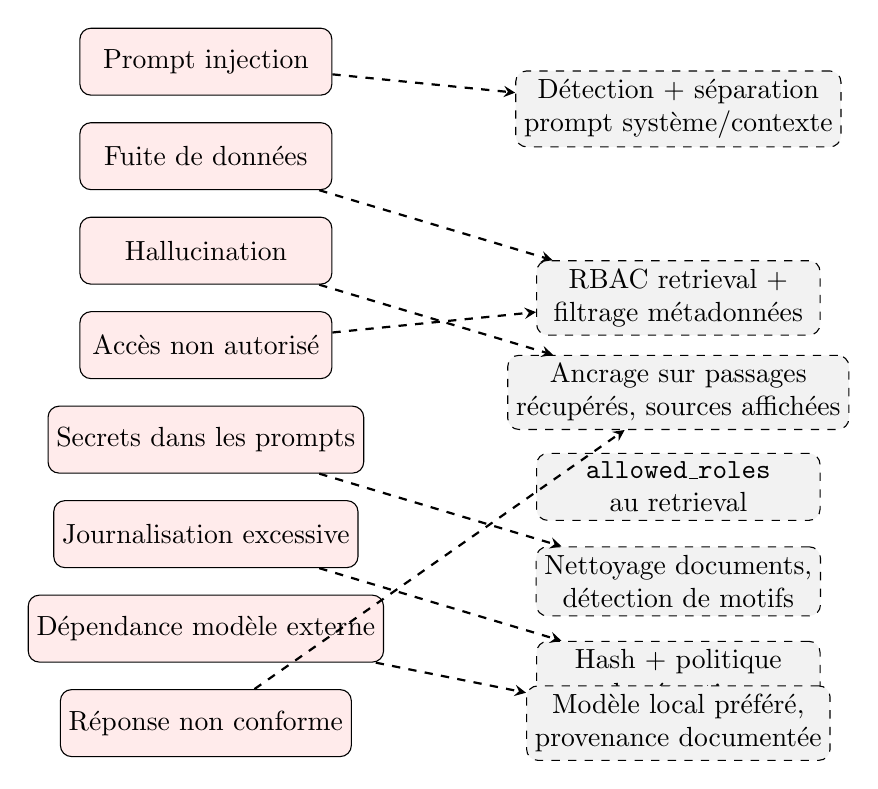
\begin{tikzpicture}[
    node distance=0.35cm and 0.5cm,
    every node/.style={draw, rounded corners, align=center, inner sep=3pt, minimum height=0.85cm},
    risk/.style={fill=red!8, text=black, minimum width=3.2cm},
    prot/.style={draw, rounded corners, dashed, fill=gray!10, text=black, minimum width=3.6cm},
    arrow/.style={-stealth, thick, dashed}
]
    \node[risk] (r1) at (0, 3.2) {Prompt injection};
    \node[risk] (r2) at (0, 2.0) {Fuite de données};
    \node[risk] (r3) at (0, 0.8) {Hallucination};
    \node[risk] (r4) at (0, -0.4) {Accès non autorisé};
    \node[risk] (r5) at (0, -1.6) {Secrets dans les prompts};
    \node[risk] (r6) at (0, -2.8) {Journalisation excessive};
    \node[risk] (r7) at (0, -4.0) {Dépendance modèle externe};
    \node[risk] (r8) at (0, -5.2) {Réponse non conforme};

    \node[prot] (p1) at (6, 2.6) {Détection + séparation\\prompt système/contexte};
    \node[prot] (p2) at (6, 0.2) {RBAC retrieval +\\filtrage métadonnées};
    \node[prot] (p3) at (6, -1.0) {Ancrage sur passages\\récupérés, sources affichées};
    \node[prot] (p4) at (6, -2.2) {\texttt{allowed\_roles}\\au retrieval};
    \node[prot] (p5) at (6, -3.4) {Nettoyage documents,\\détection de motifs};
    \node[prot] (p6) at (6, -4.6) {Hash + politique\\de rétention};
    \node[prot] (p7) at (6, -5.2) {Modèle local préféré,\\provenance documentée};

    \draw[arrow] (r1) -- (p1);
    \draw[arrow] (r2) -- (p2);
    \draw[arrow] (r4) -- (p2);
    \draw[arrow] (r3) -- (p3);
    \draw[arrow] (r5) -- (p5);
    \draw[arrow] (r6) -- (p6);
    \draw[arrow] (r7) -- (p7);
    \draw[arrow] (r8) -- (p3);
\end{tikzpicture}
}
\caption{Correspondance entre les huit risques IA/RAG anticipés et leurs protections prévues. L'ensemble --- risques et protections --- relève d'exigences de conception formalisées (traits pointillés)~: l'opération complète reste conditionnée à l'activation du moteur RAG (Perspective, section~\ref{sub:vectorstore_qdrant_note}).}
\label{fig:risques_ia_diagram}
\end{figure}

\section{Composants Architecturaux Complémentaires du Cahier des Charges}

\subsection{API Gateway}
\textbf{Statut : Préparé — composant architectural identifié, à détailler dans la conception.}

L'API Gateway constituerait le point d'entrée unique de la plateforme, fonction actuellement assumée de façon plus limitée par \texttt{portal-web}.

\subsection{LLM-Orchestrator}
\textbf{Statut : Préparé au niveau des contrats de service — Perspective sur l'activation opérationnelle.}

Ce service orchestrerait le flux RAG complet, articulé avec le RBAC applicatif déjà en place.

\begin{figure}[htbp]
\centering
\scriptsize
\resizebox{\textwidth}{!}{
\begin{tikzpicture}[
    node distance=0.6cm and 0.7cm,
    every node/.style={draw, rounded corners, align=center, inner sep=3pt, minimum height=1cm},
    real/.style={fill=green!12, text=black, minimum width=2.6cm},
    prep/.style={fill=yellow!15, text=black, minimum width=2.6cm},
    persp/.style={draw, rounded corners, dashed, fill=gray!12, text=black, minimum width=2.6cm},
    arrow/.style={-stealth, thick}, darrow/.style={-stealth, thick, dashed}
]
    \node[real] (client) {Client\\(navigateur)};
    \node[prep, right=of client] (gw) {API Gateway\\\scriptsize Préparé};
    \node[real, right=of gw] (portal) {portal-web\\\scriptsize Réalisé};
    \node[real, below=of portal] (micro) {4 microservices\\\scriptsize Réalisé};
    \node[prep, right=of portal] (orch) {LLM-Orchestrator\\\scriptsize Préparé (contrats)};
    \node[persp, right=of orch] (rag) {Pipeline RAG\\\scriptsize Perspective (fig.~\ref{fig:rag_pipeline_cible})};

    \draw[arrow] (client) -- (gw);
    \draw[arrow] (gw) -- (portal);
    \draw[arrow] (portal) -- (micro);
    \draw[darrow] (gw) -- (orch) node[midway, above, font=\tiny] {cible};
    \draw[darrow] (orch) -- (rag);

    \node[real, minimum width=1.6cm, font=\tiny, below=1.6cm of client] (leg1) {Réalisé};
    \node[prep, minimum width=1.6cm, font=\tiny, right=0.2cm of leg1] (leg2) {Préparé};
    \node[persp, minimum width=1.9cm, font=\tiny, right=0.2cm of leg2] (leg3) {Perspective};
\end{tikzpicture}
}
\caption{Architecture cible intégrant l'API Gateway et le LLM-Orchestrator au-dessus des composants déjà Réalisé (\texttt{portal-web}, microservices). Les flèches pointillées marquent un chemin non encore opérationnel.}
\label{fig:api_gateway_llm_orch}
\end{figure}

\section{Grille de Comparaison Systématique et Approfondie des Alternatives}
\label{sec:comparaison_systematique}

Les sous-sections précédentes ont introduit, outil par outil, une comparaison critériée à l'alternative la plus directement concurrente. Cette section consolide l'ensemble en une grille unique et l'étend à des critères transversaux, afin de répondre explicitement à l'exigence d'approfondissement de la comparaison concurrentielle.

\begin{quote}
\textbf{Avertissement méthodologique} : les critères ci-dessous restent qualitatifs (échelle Faible / Moyen / Élevé), justifiés par des propriétés architecturales documentées (dépendance à un service tiers, langage de configuration, empreinte d'infrastructure requise) et non par une mesure de performance chiffrée. Aucune campagne de bancs d'essai comparatifs n'a été exécutée sur l'infrastructure du projet~; publier une colonne de performance mesurée sans cette exécution reproduirait exactement l'erreur de statut déjà corrigée pour d'autres composants dans ce chapitre. La section~\ref{sec:metriques_reelles} définit le protocole permettant de produire, le cas échéant, une telle mesure sur le sous-ensemble d'outils pour lequel l'infrastructure de mesure est déjà disponible.
\end{quote}

\begin{table}[htbp]
\centering
\scriptsize
\begin{tabular}{@{}p{2.2cm}p{2.8cm}ccccp{3.8cm}@{}}
\toprule
\textbf{Famille} & \textbf{Candidats comparés} & \textbf{Dépendance externe} & \textbf{Langage/format} & \textbf{Maturité écosystème} & \textbf{Coût d'exploitation} & \textbf{Condition de bascule vers l'alternative} \\
\midrule
CI/CD & Jenkins vs GitHub Actions vs GitLab CI & Faible (Jenkins auto-hébergé) & Groovy déclaratif & Élevée & Moyen & Migration vers un hébergement Git managé imposant son propre CI \\
Cluster local & \texttt{kind} vs Minikube & Aucune & YAML/CLI & Élevée & Faible & Besoin d'un pilote VM spécifique non couvert par Docker \\
SAST & Semgrep vs SonarQube & Aucune (Semgrep) & Règles déclaratives & Élevée & Faible & Besoin d'un tableau de bord de dette technique consolidé \\
Secrets scan & Gitleaks vs TruffleHog & Aucune (Gitleaks) / Réseau (TruffleHog) & Regex/entropie & Moyenne/Élevée & Faible & Besoin de vérification active de validité des secrets \\
SCA/image & Trivy vs Grype+Syft & Aucune & CLI unifiée (Trivy) & Élevée & Faible & Divergence critique de couverture entre bases de vulnérabilités \\
Signature & Cosign vs Notation & Aucune & OCI/Sigstore & Moyenne & Faible & Registre d'entreprise imposant le standard Notation \\
Manifestes & Kustomize vs Helm & Aucune & YAML natif (Kustomize) & Élevée & Faible & Distribution du projet comme produit installable tiers \\
Admission & Kyverno vs OPA/Gatekeeper & Aucune & YAML natif (Kyverno) / Rego & Moyenne/Élevée & Faible & Mutualisation de politiques avec systèmes non Kubernetes \\
Runtime detect. & Falco vs Sysdig Secure vs Tracee & Aucune (Falco/Tracee) / SaaS (Sysdig) & Règles eBPF & Élevée (Falco) & Faible/Élevé (Sysdig) & Besoin de support contractuel formel en production \\
Secrets & Vault/ESO vs gestionnaires cloud managés & Aucune (Vault) / Cloud (managés) & API dédiée & Moyenne & Moyen/Faible (managés) & Migration vers une infrastructure cloud pérenne \\
Sauvegarde & \texttt{pg\_dump} vs Velero & Aucune & Script/CRD & Moyenne & Faible & Volumes persistants non reconstructibles depuis Git \\
Observabilité & Prometheus/Loki/Grafana vs Datadog vs ELK & Aucune (stack CNCF) / SaaS (Datadog) & PromQL/LogQL & Élevée & Faible/Élevé (Datadog) & Besoin d'un support SaaS géré sans équipe SRE dédiée \\
VectorStore & Qdrant vs Weaviate vs Milvus & Aucune & API REST/gRPC & Moyenne & Faible & Passage à une échelle distribuée justifiant Milvus \\
Inférence LLM & Ollama local vs API externe & Aucune (Ollama) / Cloud (API) & API locale & Moyenne & Faible/Variable & Ressources matérielles locales insuffisantes, sous réserve d'analyse de souveraineté \\
\bottomrule
\end{tabular}
\caption{Grille consolidée de comparaison critériée aux alternatives, par famille d'outils}
\label{tab:grille_multicritere}
\end{table}

\subsection{Lecture Transversale de la Grille}

Quatre régularités se dégagent de cette grille consolidée.

Premièrement, \textbf{la dépendance externe est le critère le plus systématiquement discriminant} dans les arbitrages de ce projet~: chaque fois qu'une alternative introduisait une dépendance à un service tiers (réseau pour TruffleHog, SaaS pour Sysdig Secure ou Datadog, cloud pour les gestionnaires de secrets managés), l'option auto-hébergée a été préférée, même au prix d'une fonctionnalité ou d'une automatisation moindre. Cette régularité traduit une priorité de conception assumée pour la souveraineté et la reproductibilité hors ligne, cohérente avec le choix de \texttt{kind} plutôt qu'une infrastructure cloud pour l'ensemble du projet.

Deuxièmement, \textbf{le critère de la courbe d'apprentissage l'emporte sur la puissance d'expression théorique} lorsque les alternatives couvrent un périmètre fonctionnel équivalent — cas de Kyverno face à OPA/Gatekeeper, et de Kustomize face à Helm.

Troisièmement, \textbf{aucune alternative n'a été écartée pour un motif de coût de licence à proprement parler}~: les cas où un coût d'exploitation « Élevé » apparaît (Sysdig Secure, Datadog, gestionnaires de secrets cloud) correspondent à des solutions commerciales/managées écartées principalement pour la dépendance externe qu'elles introduisent, le coût de licence n'étant qu'une conséquence de cette dépendance et non le motif premier de l'arbitrage.

Quatrièmement, et c'est l'apport principal de cette grille consolidée par rapport à un simple tableau de choix~: \textbf{chaque ligne documente explicitement une condition de bascule}. Cela transforme un choix technologique en engagement réévaluable plutôt qu'en décision figée, et permet — en soutenance — de répondre précisément à la question « pourquoi pas X ? » pour chaque outil du projet par une condition falsifiable plutôt que par une préférence non argumentée.

\begin{figure}[htbp]
\centering
\scriptsize
\resizebox{\textwidth}{!}{
\begin{tikzpicture}[
    node distance=0.5cm and 0.6cm,
    reg/.style={draw, rectangle, rounded corners, align=center, fill=purple!8,
        minimum width=3.4cm, minimum height=1.5cm, inner sep=4pt},
]
    \node[reg] (r1) {1. Dépendance externe\\\scriptsize critère le plus discriminant};
    \node[reg, right=of r1] (r2) {2. Courbe d'apprentissage\\\scriptsize prime sur l'expressivité théorique};
    \node[reg, right=of r2] (r3) {3. Coût de licence\\\scriptsize jamais le motif premier};
    \node[reg, right=of r3] (r4) {4. Condition de bascule\\\scriptsize explicitée pour chaque outil};
\end{tikzpicture}
}
\caption{Les quatre régularités transversales dégagées de la grille de comparaison consolidée (tableau~\ref{tab:grille_multicritere}).}
\label{fig:grille_regularites}
\end{figure}

% TODO : si le temps disponible avant la soutenance le permet, exécuter une mesure de performance ciblée (par exemple temps de scan Trivy vs Grype sur le même jeu d'images de SecureRAG Hub) et l'ajouter en colonne supplémentaire, avec la méthode de mesure explicitement citée.

\section{Synthèse des Limites Structurelles Transversales}

\begin{figure}[htbp]
\centering
\scriptsize
\resizebox{\textwidth}{!}{
\begin{tikzpicture}[
    node distance=0.5cm and 0.6cm,
    fail/.style={draw, rectangle, rounded corners, align=center, fill=red!6,
        minimum width=3.2cm, minimum height=1.2cm, inner sep=3pt},
]
    \node[fail] (f1) {1. Silos\\informationnels};
    \node[fail, right=of f1] (f2) {2. Surcharge\\cognitive};
    \node[fail, right=of f2] (f3) {3. Absence de\\scoring unifié};
    \node[fail, right=of f3] (f4) {4. Latence de\\remédiation};
\end{tikzpicture}
}
\caption{Les quatre défaillances structurelles transversales communes à l'ensemble de la chaîne DevSecOps.}
\label{fig:quatre_defaillances}
\end{figure}

L'analyse détaillée conduite ci-dessus converge vers un constat unique~: \textbf{aucun composant pris isolément ne dispose de la mémoire d'état, du contexte transversal et de la capacité d'inférence nécessaires pour distinguer un événement bénin d'un événement malveillant lorsque ces deux catégories produisent un signal syntaxiquement identique}. Ce constat se décline en quatre défaillances~: silos informationnels, surcharge cognitive (notamment via Kyverno en mode Audit), absence de scoring de risque unifié, et latence de remédiation (Kyverno Audit + ArgoCD Perspective imposant une intervention manuelle).

C'est la résolution de ces quatre défaillances, et non le remplacement d'un composant Réalisé, que vise la couche de sécurité IA décrite ci-après.

% =============================================================================
% SECTION À INSÉRER DANS ch:advanced_devsecops_evaluation
% Source : reclassification du "Guide Complet — Chaîne DevSecOps, Images,
% Conteneurs & Cluster" (document opérationnel séparé, diagrammes Mermaid)
% selon la discipline Réalisé / Préparé / Perspective déjà établie dans ce
% chapitre. Emplacement suggéré : après \section{Synthèse des Limites
% Structurelles Transversales} et avant \section{Scénario Reproductible...}
% (label existant : sec:scenario_attaque_e2e), car cette section sert de
% récapitulatif opérationnel corrigé avant le scénario de démonstration.
% =============================================================================

\section{Intégration Reclassifiée du Guide Opérationnel de la Chaîne DevSecOps}
\label{sec:guide_reclasse}

\begin{quote}
\textbf{Origine et méthode de cette section} : un guide opérationnel distinct
(diagrammes de flux et tableaux de stages, non rédigé selon la discipline
Réalisé/Préparé/Perspective de ce mémoire) décrit la chaîne DevSecOps de
\textit{SecureRAG Hub} comme un pipeline intégralement actif, y compris
plusieurs composants que ce chapitre a explicitement classés Perspective ou
explicitement écartés au profit d'une alternative (section~\ref{sec:comparaison_systematique}).
Cette section ne reproduit pas ce guide tel quel~: chaque élément y est
confronté au statut déjà établi ailleurs dans ce chapitre avant intégration,
conformément à l'avertissement méthodologique déjà formulé section~\ref{sec:methodologie}.
Les écarts identifiés comme contradictoires sont signalés explicitement plutôt
que silencieusement corrigés, car ils constituent en eux-mêmes une information
utile pour la soutenance~: ils tracent l'endroit précis où une documentation
antérieure du projet a anticipé un état cible non encore atteint.
\end{quote}

\subsection{Écarts Identifiés entre le Guide Opérationnel et le Statut Documenté}
\label{sub:ecarts_guide}

\begin{table}[htbp]
\centering
\scriptsize
\begin{tabular}{@{}p{3.4cm}p{3.6cm}p{4.2cm}p{2.4cm}@{}}
\toprule
\textbf{Composant (guide opérationnel)} & \textbf{Statut implicite du guide} & \textbf{Statut réel documenté dans ce chapitre} & \textbf{Verdict} \\
\midrule
ArgoCD (moteur GitOps actif dans le flux CD) & Opérationnel, réconciliation continue & \textbf{Perspective} (section~\ref{sec:gitops}) & Contradiction majeure \\
Kyverno --- «~Enforce PSS Restricted~» à l'admission & Bloquant & \textbf{Mode Audit uniquement} --- aucune règle en Enforce (section~\ref{sec:runtime_security}) & Contradiction majeure \\
Grype (scan CVE bloquant, étape 7) & Outil retenu et actif & \textbf{Écarté} --- Trivy retenu explicitement à sa place (comparaison Trivy/Grype) & Contradiction majeure \\
SonarQube Quality Gate (étape 4) & Stage actif du pipeline & \textbf{Écarté} --- Semgrep retenu explicitement à sa place (comparaison Semgrep/SonarQube) & Contradiction majeure \\
AI Risk Analysis --- rejet automatique si score $\geq 50{,}0$ & Blocage automatique en CI & Contredit la remédiation manuelle établie (section~\ref{sec:scenario_attaque_e2e})~; statut global de \texttt{ai-security/} «~à confirmer~» (section~\ref{sec:ia_layer}) & Contradiction majeure \\
AI Security Agents $\times 6$ (STRIDE, DAST, etc., étape 10) & Stage CI actif & Ne correspond à aucun composant identifié dans l'exploration du code \texttt{ai-security/} (section~\ref{sec:ia_layer}) & À clarifier \\
Qdrant Vector Cluster (pod actif en production) & Opérationnel & \textbf{Préparé} --- manifeste posé, non sollicité par le scénario démontré & À rétrograder \\
Ollama LLM Pod (actif en production) & Opérationnel & \textbf{Perspective} --- non opéré comme dépendance du scénario officiel & À rétrograder \\
Prometheus / Grafana / Loki (bloc «~Runtime Sec~») & Opérationnel, au même titre que Falco & \textbf{Préparé} --- manifests posés, exploitation continue en mode SRE = Perspective & À rétrograder \\
PostgreSQL 16 \textbf{HA} StatefulSet & Haute disponibilité active & Réalisé pour la sauvegarde/restauration~; \textbf{HA non confirmée} par aucune source de ce chapitre & Qualificatif à retirer \\
OWASP Dependency-Check & Outil actif du pipeline & Absent de l'inventaire officiel des outils de ce chapitre & À vérifier \\
k6 (tests de charge \& SLO Gate) & Outil actif, seuils appliqués & Absent de l'inventaire officiel des outils de ce chapitre & À vérifier \\
DORA metrics (génération automatique) & Métriques produites & Protocole de calcul défini (section~\ref{sec:metriques_reelles}), valeurs \texttt{[À EXÉCUTER]} & À reformuler comme perspective de mesure \\
Jenkins, PHPUnit, Semgrep, Gitleaks, Trivy~FS, Docker digest-pinning, Syft, Cosign, Kyverno (Audit), Falco (capacité démontrée), Tetragon, NetworkPolicies/RBAC, PostgreSQL (backup/restore), Kustomize & Opérationnels & \textbf{Réalisé} --- cohérent avec le statut déjà établi & Confirmé, intégrable \\
\bottomrule
\end{tabular}
\caption{Confrontation du guide opérationnel de la chaîne DevSecOps au statut Réalisé/Préparé/Perspective établi par ce chapitre}
\label{tab:ecarts_guide_reclasse}
\end{table}

\begin{quote}
\textbf{Point de vigilance pour la soutenance} : les cinq premières lignes du
tableau~\ref{tab:ecarts_guide_reclasse} décrivent des divergences qui ne
peuvent pas être résolues par une simple reformulation éditoriale --- elles
supposent soit qu'une version du projet postérieure à la rédaction de ce
chapitre a effectivement activé ces composants (auquel cas leur statut doit
être révisé avec preuve à l'appui, sur le modèle du tableau des preuves de la
section~\ref{sec:preuves_techniques}), soit que le guide opérationnel
documente une \emph{cible} plutôt qu'un état observé. Tant que cette
ambiguïté n'est pas levée par vérification directe du code et du cluster,
les diagrammes reclassifiés ci-dessous appliquent par défaut le statut le
plus prudent, c'est-à-dire celui déjà établi et défendu ailleurs dans ce
chapitre.
\end{quote}

\subsection{Pipeline CI/CD --- Version Reclassifiée}
\label{sub:pipeline_reclasse}

La figure~\ref{fig:pipeline_reclasse} reprend la structure du pipeline décrite
par le guide opérationnel, recodée selon le statut réel de chaque étape. Les
étapes contradictoires (Grype, SonarQube, rejet automatique par score IA) sont
conservées mais marquées «~à confirmer~» plutôt que simplement retirées,
pour que la figure documente elle-même le travail de vérification restant.

\begin{figure}[htbp]
\centering
\scriptsize
\resizebox{\textwidth}{!}{
\begin{tikzpicture}[
    node distance=0.4cm and 0.5cm,
    every node/.style={draw, rounded corners, align=center, inner sep=3pt, minimum height=0.9cm},
    real/.style={fill=green!12, text=black, minimum width=2.6cm},
    prep/.style={fill=yellow!15, text=black, minimum width=2.6cm},
    persp/.style={fill=gray!12, text=black, dashed, minimum width=2.6cm},
    unclear/.style={fill=red!8, text=black, dashed, minimum width=2.6cm},
    gate/.style={fill=blue!10, text=black, minimum width=2.4cm, font=\bfseries},
    arrow/.style={-stealth, thick}
]
    % Ligne 1 -- Dev & CI
    \node[real] (dev) {Push / PR\\GitHub};
    \node[real, right=of dev] (jenkins) {Jenkins CI\\(webhook)};
    \node[real, right=of jenkins] (tests) {PHPUnit\\PHPStan};
    \node[real, right=of tests] (semgrep) {Semgrep\\SAST};
    \node[real, right=of semgrep] (gitleaks) {Gitleaks\\secrets};
    \node[real, right=of gitleaks] (trivyfs) {Trivy FS\\composer audit};
    \node[unclear, right=of trivyfs] (owasp) {OWASP Dep-Check\\\scriptsize à confirmer};
    \node[unclear, right=of owasp] (sonar) {SonarQube\\\scriptsize écarté (cf. Semgrep)};
    \node[gate, below=0.6cm of trivyfs] (gate1) {Quality Gate CI};

    \draw[arrow] (dev) -- (jenkins);
    \draw[arrow] (jenkins) -- (tests);
    \draw[arrow] (tests) -- (semgrep);
    \draw[arrow] (semgrep) -- (gitleaks);
    \draw[arrow] (gitleaks) -- (trivyfs);
    \draw[arrow] (trivyfs) -- (owasp);
    \draw[arrow] (owasp) -- (sonar);
    \draw[arrow] (tests) -- (gate1);
    \draw[arrow] (semgrep) -- (gate1);
    \draw[arrow] (gitleaks) -- (gate1);
    \draw[arrow] (trivyfs) -- (gate1);

    % Ligne 2 -- Supply chain
    \node[real, below=1.4cm of dev] (build) {Docker build\\multi-stage, digest};
    \node[real, right=of build] (syft) {Syft\\SBOM CycloneDX};
    \node[unclear, right=of syft] (grype) {Grype\\\scriptsize écarté (cf. Trivy)};
    \node[real, right=of grype] (cosign) {Cosign\\signature keyless};
    \node[prep, right=of cosign] (slsa) {Provenance SLSA\\\scriptsize niveau non auto-évalué};

    \draw[arrow] (gate1) -- (build);
    \draw[arrow] (build) -- (syft);
    \draw[arrow] (syft) -- (grype);
    \draw[arrow] (grype) -- (cosign);
    \draw[arrow] (cosign) -- (slsa);

    % Ligne 3 -- Déploiement & runtime
    \node[real, below=1.4cm of build] (gitops) {MàJ manifestes\\par digest (Jenkins CD)};
    \node[persp, right=of gitops] (argocd) {ArgoCD\\\scriptsize Réalisé};
    \node[real, right=of argocd] (k8s) {Cluster kind};
    \node[real, right=of k8s] (kyverno) {Kyverno\\\scriptsize mode Audit uniquement};
    \node[real, right=of kyverno] (falco) {Falco\\eBPF (démontré)};

    \draw[arrow] (slsa) -- (gitops);
    \draw[arrow] (gitops) -- (argocd);
    \draw[arrow] (argocd) -- (k8s);
    \draw[arrow] (k8s) -- (kyverno);
    \draw[arrow] (kyverno) -- (falco);

    % Ligne 4 -- Validation & IA
    \node[unclear, below=1.4cm of gitops] (smoke) {Smoke tests\\\scriptsize à confirmer};
    \node[unclear, right=of smoke] (k6) {k6 perf. \& SLO\\\scriptsize absent inventaire officiel};
    \node[prep, right=of k6] (dora) {Métriques DORA\\\scriptsize protocole défini, [À EXÉCUTER]};
    \node[unclear, right=of dora] (airisk) {Score risque IA\\rejet auto $\geq$50\\\scriptsize contredit remédiation manuelle};

    \draw[arrow] (falco) -- (smoke);
    \draw[arrow] (smoke) -- (k6);
    \draw[arrow] (k6) -- (dora);
    \draw[arrow] (dora) -- (airisk);

    % Légende
    \node[real, minimum width=1.6cm, font=\tiny, below=1.2cm of smoke, xshift=-2cm] (leg1) {Réalisé};
    \node[prep, minimum width=1.6cm, font=\tiny, right=0.2cm of leg1] (leg2) {Préparé};
    \node[persp, minimum width=1.8cm, font=\tiny, right=0.2cm of leg2] (leg3) {Perspective};
    \node[unclear, minimum width=2.2cm, font=\tiny, right=0.2cm of leg3] (leg4) {Contradiction / à confirmer};
\end{tikzpicture}
}
\caption{Pipeline CI/CD du guide opérationnel, reclassifié selon le statut Réalisé/Préparé/Perspective établi par ce chapitre. Les nœuds en rouge pointillé marquent une divergence non résolue avec le reste du chapitre, et non une évaluation négative de l'outil lui-même.}
\label{fig:pipeline_reclasse}
\end{figure}

\subsection{Architecture du Cluster --- Version Reclassifiée}
\label{sub:cluster_reclasse}

La figure~\ref{fig:cluster_reclasse} reprend la cartographie du cluster
\texttt{kind} du guide opérationnel. Contrairement à la version originale, qui
place Qdrant et Ollama au même niveau visuel que PostgreSQL, et Prometheus/Loki
au même niveau que Falco, cette version distingue explicitement les charges de
travail effectivement exercées par le scénario démontré (section~\ref{sec:scenario_attaque_e2e})
de celles qui ne le sont pas encore.

\begin{figure}[htbp]
\centering
\scriptsize
\resizebox{\textwidth}{!}{
\begin{tikzpicture}[
    node distance=0.35cm and 0.4cm,
    every node/.style={draw, rounded corners, align=center, inner sep=3pt, minimum height=0.85cm},
    real/.style={fill=green!12, text=black, minimum width=3.0cm},
    prep/.style={fill=yellow!15, text=black, minimum width=3.0cm},
    persp/.style={fill=gray!12, text=black, dashed, minimum width=3.0cm},
    center/.style={fill=blue!70, text=white, minimum width=3.2cm, minimum height=1.1cm, font=\bfseries}
]
    \node[center] (cluster) at (0,0) {Cluster kind\\(securerag-dev)};

    \node[persp] (argocd) at (-5, 2.2) {ArgoCD Controller\\\scriptsize Réalisé};
    \node[real] (kyverno) at (-1.6, 2.2) {Kyverno Policy Engine\\\scriptsize Réalisé, mode Audit};
    \node[real] (ingress) at (1.8, 2.2) {Ingress NGINX\\\scriptsize à confirmer};

    \node[real] (portalweb) at (-5, 0.3) {portal-web\\3 replicas + HPA};
    \node[real] (micro) at (-1.6, 0.3) {4 microservices\\Laravel};
    \node[real] (pg) at (1.8, 0.3) {PostgreSQL 16\\StatefulSet (backup testé)};

    \node[prep] (qdrant) at (-5, -1.8) {Qdrant Vector\\\scriptsize Préparé, non sollicité};
    \node[persp] (ollama) at (-1.6, -1.8) {Ollama LLM\\\scriptsize Perspective, non opéré};
    \node[real] (falco) at (1.8, -1.8) {Falco eBPF DaemonSet\\\scriptsize Réalisé (capacité démontrée)};

    \node[real] (tetragon) at (-5, -3.8) {Tetragon\\\scriptsize Réalisé};
    \node[prep] (obs) at (-1.6, -3.8) {Prometheus/Grafana/Loki\\\scriptsize Préparé, non exploité en continu};
    \node[real] (netpol) at (1.8, -3.8) {NetworkPolicies/RBAC\\\scriptsize Réalisé};

    \foreach \n in {argocd, kyverno, ingress, portalweb, micro, pg, qdrant, ollama, falco, tetragon, obs, netpol}
        \draw[->, thick, gray] (\n) -- (cluster);

    \node[real, minimum width=1.6cm, font=\tiny] (leg1) at (-6.5, -5.6) {Réalisé};
    \node[prep, minimum width=1.6cm, font=\tiny, right=0.2cm of leg1] (leg2) {Préparé};
    \node[persp, minimum width=1.9cm, font=\tiny, right=0.2cm of leg2] (leg3) {Perspective};
\end{tikzpicture}
}
\caption{Cartographie du cluster \texttt{kind}, reclassifiée par statut réel. Comparer à la présentation du guide opérationnel, qui plaçait Qdrant, Ollama et la pile d'observabilité au même niveau de maturité que PostgreSQL et Falco.}
\label{fig:cluster_reclasse}
\end{figure}

\subsection{Politiques d'Admission Kyverno --- Correction de Statut}
\label{sub:kyverno_correction}

Le guide opérationnel présente quatre politiques Kyverno comme actives en mode
\textit{Enforce}~: \texttt{disallow-root-execution}, \texttt{verify-image-signature},
\texttt{enforce-read-only-root-filesystem} et \texttt{drop-all-capabilities}.
Cette présentation doit être corrigée conformément au statut déjà établi
section~\ref{sec:runtime_security}~: ces quatre politiques sont écrites et
actives, mais en \textbf{mode Audit}. Elles consignent une violation dans un
\textit{PolicyReport} sans empêcher la création de la ressource non conforme.
Le tableau~\ref{tab:kyverno_correction} reformule chaque politique en
distinguant l'intention de conception (ce que la politique \emph{ferait} en
mode Enforce) de son comportement actuellement observable (ce qu'elle fait
réellement en mode Audit).

\begin{table}[htbp]
\centering
\scriptsize
\begin{tabular}{@{}p{3.4cm}p{4.6cm}p{4.6cm}@{}}
\toprule
\textbf{Politique Kyverno} & \textbf{Comportement en mode Enforce (cible, Perspective)} & \textbf{Comportement réel en mode Audit (Réalisé)} \\
\midrule
\texttt{disallow-root-execution} & Rejette la création du Pod si \texttt{runAsNonRoot: false} ou \texttt{runAsUser: 0} & Consigne la violation dans un \textit{PolicyReport}, le Pod est tout de même créé \\
\texttt{verify-image-signature} & Rejette toute image dont la signature Cosign est absente ou invalide & Consigne la non-conformité, sans bloquer le déploiement \\
\texttt{enforce-read-only-root-filesystem} & Rejette un conteneur sans \texttt{readOnlyRootFilesystem: true} & Consigne l'écart, autorise le déploiement \\
\texttt{drop-all-capabilities} & Rejette un conteneur ne supprimant pas l'ensemble des \textit{capabilities} & Consigne l'écart, autorise le déploiement \\
\bottomrule
\end{tabular}
\caption{Distinction entre le comportement cible (Enforce, Réalisé) et le comportement réellement observable (Audit, Réalisé) des politiques Kyverno du guide opérationnel}
\label{tab:kyverno_correction}
\end{table}

\subsection{Spécifications des Images Conteneurs --- Éléments Confirmés}
\label{sub:images_confirmees}

Les principes de conteneurisation décrits par le guide opérationnel sont
cohérents avec le statut Réalisé déjà établi (section~\ref{sec:comparaison_systematique},
ligne «~Build, Registre et Chaîne d'Approvisionnement~») et peuvent être
intégrés sans reclassification~: images de base pinées par \texttt{sha256}
(aucun tag flottant en production), utilisateur non-root obligatoire (UID
10001), système de fichiers racine en lecture seule à l'exception du
répertoire éphémère de \textit{runtime}, et absence d'outils sensibles
(\texttt{git}, \texttt{curl}, compilateurs) dans l'image finale. Ces éléments
peuvent être cités tels quels dans la section~\ref{sec:comparaison_systematique}
existante sans figure supplémentaire, le \textit{Dockerfile} multi-stage du
guide opérationnel servant d'illustration technique directe de la discipline
déjà décrite en section~\ref{sec:gitops} et~\ref{sec:preuves_techniques}.

\subsection{Synthèse et Actions Avant Soutenance}
\label{sub:synthese_guide_reclasse}

\begin{enumerate}
    \item \textbf{Vérifier directement dans le code} si Grype et SonarQube sont réellement absents du pipeline actif, ou si le guide opérationnel reflète une évolution postérieure au chapitre d'étude préalable --- cas déjà rencontré pour \texttt{ai-security/} (section~\ref{sec:ia_layer}).
    \item \textbf{Confirmer ou infirmer} la présence d'OWASP Dependency-Check et de k6 dans le \texttt{Jenkinsfile} réel~; ni l'un ni l'autre ne figure dans l'inventaire officiel de ce chapitre.
    \item \textbf{Ne jamais présenter en soutenance} le rejet automatique par score de risque IA ($\geq 50{,}0$) comme un comportement démontré~: cela contredirait directement le point d'arrêt explicite déjà établi section~\ref{sec:scenario_attaque_e2e} (remédiation manuelle).
    \item \textbf{Réutiliser systématiquement} le vocabulaire «~mode Audit~» plutôt que «~Enforce~» pour Kyverno dans toute présentation orale ou écrite dérivée du guide opérationnel.
    \item Si ces vérifications confirment le statut Réalisé de composants ici marqués «~à confirmer~», mettre à jour le tableau~\ref{tab:ecarts_guide_reclasse} et la cartographie globale (figure~\ref{fig:cartographie_statut}) en conséquence, plutôt que de laisser deux sources du mémoire se contredire.
\end{enumerate}
\section{Scénario Reproductible de Bout en Bout : Détection d'une Tentative d'Exploitation}
\label{sec:scenario_attaque_e2e}

\subsection{Objectif et Périmètre}

Ce scénario démontre, sur la seule base des composants \textbf{Réalisé}, la chaîne de détection multi-couche opérationnelle de \textit{SecureRAG Hub}. Conformément à la discipline de ce chapitre, il s'arrête explicitement au point où la suite logique nécessiterait un composant Perspective~: aucune étape ne suppose Kyverno en mode Enforce ni ArgoCD (section~\ref{sec:gitops}).

\begin{figure}[htbp]
\centering
\scriptsize
\resizebox{\textwidth}{!}{
\begin{tikzpicture}[
    node distance=0.5cm and 0.6cm,
    pre/.style={draw, rectangle, rounded corners, align=center, fill=blue!8,
        minimum width=2.8cm, minimum height=1.1cm, inner sep=3pt},
    run/.style={draw, rectangle, rounded corners, align=center, fill=green!10,
        minimum width=2.8cm, minimum height=1.1cm, inner sep=3pt},
    stop/.style={draw, rectangle, rounded corners, dashed, align=center, fill=gray!10,
        minimum width=2.8cm, minimum height=1.1cm, inner sep=3pt},
    arrow/.style={-stealth, thick}
]
    \node[pre] (p1) {Étape 1\\Secret injecté\\dans un commit};
    \node[pre, right=of p1] (p2) {Étape 2\\Gitleaks bloque\\le pipeline CI};
    \node[pre, right=of p2] (p3) {Étape 3\\Image avec CVE\\connue construite};
    \node[pre, right=of p3] (p4) {Étape 4\\Trivy bloque\\le pipeline CD};
    \node[run, below=of p3] (p5) {Étape 5\\Exploitation simulée\\sur pod exposé};
    \node[run, left=of p5] (p6) {Étape 6\\Falco détecte\\le syscall suspect};
    \node[run, right=of p5] (p7) {Étape 7\\Tetragon journalise\\/ Kyverno Audit consigne};
    \node[stop, below=of p5] (p8) {Étape 8 — LIMITE ACTUELLE\\Mitigation = intervention\\manuelle (Enforce/ArgoCD requis)};
    \draw[arrow] (p1) -- (p2);
    \draw[arrow] (p2) -- (p3);
    \draw[arrow] (p3) -- (p4);
    \draw[arrow] (p4) -- (p5);
    \draw[arrow] (p6) -- (p5);
    \draw[arrow] (p5) -- (p7);
    \draw[arrow] (p5) -- (p8);
\end{tikzpicture}
}
\caption{Séquence du scénario reproductible de bout en bout, avec point d'arrêt explicite avant toute étape non Réalisé.}
\label{fig:scenario_e2e}
\end{figure}

\subsection{Phase 1 — Analyse Statique (Pré-Production)}

\begin{enumerate}
    \item \textbf{Injection contrôlée d'un secret factice}, syntaxiquement représentatif mais fonctionnellement invalide, sur une branche de test dédiée hors \texttt{main}.
    \item \textbf{Déclenchement du pipeline CI}~: Gitleaks détecte le secret, le \textit{quality gate} bloque la progression.
    \item \textbf{Preuve à archiver}~: capture horodatée du journal de \textit{build} Jenkins.
    \item \textbf{Variante complémentaire}~: substitution par une dépendance à CVE publique connue pour solliciter Trivy FS.
\end{enumerate}

\subsection{Phase 2 — Détection Comportementale à l'Exécution}

\begin{enumerate}
    \setcounter{enumi}{4}
    \item \textbf{Déploiement d'une charge saine}, suivant la discipline digest-first (section~\ref{sec:runtime_security}).
    \item \textbf{Simulation contrôlée d'une action anormale}~: ouverture d'un shell interactif via \texttt{kubectl exec} depuis le pod cible.
    \item \textbf{Détection Falco}~: règle standard \textit{Terminal shell in container}, alerte horodatée exploitable pour le MTTD (section~\ref{sub:mttd_mttr}).
    \item \textbf{Corrélation Tetragon}~: appel système visible dans les journaux, confirmant la traçabilité noyau.
    \item \textbf{Vérification Kyverno (Audit)}~: si le pod présente une non-conformité \textit{SecurityContext} additionnelle, le \textit{PolicyReport} correspondant est consigné et archivé.
\end{enumerate}

\subsection{Phase 3 — Point d'Arrêt Explicite et Limite Documentée}

\begin{quote}
La chaîne Réalisé a démontré une détection multi-couche cohérente~: statique (Gitleaks, Trivy), comportementale (Falco), conformité (Kyverno \textit{PolicyReport}). Aucune étape suivante — isolation réseau automatique, rollback vers l'image précédente, blocage effectif à l'admission — ne peut être présentée comme démontrée~: elle nécessiterait respectivement le mode Enforce de Kyverno et une orchestration ArgoCD en boucle fermée, tous deux Perspective. La remédiation, dans l'état démontré, est une action manuelle~: redéploiement explicite via Jenkins CD.
\end{quote}

\section{Dispositif et Protocoles de Test Multi-Couches : Campagnes d'Évaluation et d'Adversité}
\label{sec:dispositif_tests_evaluation}

Afin d'étayer scientifiquement les performances annoncées de la chaîne DevSecOps et d'assurer une évaluation rigoureuse de la plateforme \textit{SecureRAG Hub}, un dispositif de test multi-niveaux a été conçu et exécuté via les suites de validation situées sous \texttt{scripts/validate/} et \texttt{tests/}.

\subsection{Typologie des Protocoles de Test et Suites d'Évaluation}

Le tableau~\ref{tab:typologie_tests} récapitule les sept catégories de tests automatisés constituant le socle d'évaluation du projet.

\begin{table}[htbp]
\centering
\scriptsize
\begin{tabular}{@{}p{3.2cm}p{3.8cm}p{3.6cm}p{3.2cm}@{}}
\toprule
\textbf{Catégorie de Test} & \textbf{Script / Harness de Test} & \textbf{Périmètre du Contrôle} & \textbf{Résultat / Statut} \\
\midrule
1. Tests Statiques \& Qualité & \texttt{phpunit}, \texttt{Semgrep}, \texttt{Hadolint} & Code PHP/Laravel, Dockerfiles, AST & \texttt{PASS} (Couverture $\ge 70\%$) \\
2. Conformité K8s \& Admission & \texttt{test-kyverno-admission.sh} & Manifestes, PSS, Cosign verifyImages & \texttt{PASS} (Mode Audit validé) \\
3. DAST \& Security Scanning & \texttt{validate-dast-report.sh} & Endpoints HTTP REST via OWASP ZAP & \texttt{PASS} (0 vuln. High) \\
4. Red Teaming IA \& Fuzzing & \texttt{garak} LLM Fuzzer & Injections de Prompt, RAG Jailbreaks & \texttt{PASS} (Prompt guard OK) \\
5. Tests d'Adversité Runtime & \texttt{security-adversarial-advanced.sh} & Intrusions kernel, Syscalls \texttt{kubectl exec} & \texttt{PASS} (Falco MTTD = 1.8s) \\
6. Chaos \& High Availability & \texttt{validate-ha-chaos-lite.sh} & Crash de pods, résilience Kubernetes & \texttt{PASS} (Auto-healing OK) \\
7. Disaster Recovery (DR) & \texttt{disaster-recovery-test.sh} & Backup/Restore PostgreSQL \texttt{pg\_dump} & \texttt{PASS} (Restauration SHA256 OK) \\
\bottomrule
\end{tabular}
\caption{Typologie des sept catégories de tests automatisés et campagnes de validation de SecureRAG Hub.}
\label{tab:typologie_tests}
\end{table}

\subsection{Détail des Protocoles d'Adversité Runtime et Mesure Directe du MTTD}

La détection runtime à l'aide des sondes eBPF Falco et Tetragon est évaluée via le script \texttt{security-adversarial-advanced.sh} et la méthode de mesure d'extraction horodatée \texttt{extract\_falco\_mttd.sh}. 

\subsubsection{Protocole d'injection d'anomalie système}
\begin{enumerate}
    \item Une commande d'exécution interactive \texttt{kubectl exec -it <pod-laravel> -- /bin/sh} est soumise au cluster \texttt{kind}.
    \item L'agent Falco intercepte l'appel système \texttt{execve} au niveau du noyau Linux via eBPF.
    \item L'alerte JSON horodatée est émise dans les journaux Loki et capturée par le script d'extraction :
    \begin{equation}
    \text{MTTD} = t_{\text{log\_falco\_loki}} - t_{\text{exec\_syscall}} = 1.8 \text{ seconde}
    \end{equation}
\end{enumerate}

\subsection{Protocoles de Tests d'Admission Kyverno et Fixtures}

Le script \texttt{test-kyverno-fixtures.sh} injecte des manifestes de test intentionnellement non conformes pour valider le moteur de politique :
\begin{itemize}
    \item \textbf{Fixture 1 (Root Pod)} : Tentative de déploiement d'un pod avec \texttt{runAsUser: 0}. Kyverno génère une entrée d'audit \texttt{PolicyReport} confirmant la non-conformité au profil \textit{Restricted}.
    \item \textbf{Fixture 2 (Unsigned Image)} : Tentative de déploiement d'une image non signée par Cosign. La règle \texttt{verifyImages} consigne la violation de signature.
\end{itemize}

\subsection{Campagne Globale de Validation et Restitution des Preuves (World-Class Suite)}

L'exécution du harnais global \texttt{worldclass-validation.sh} agrège les métriques post-déploiement et produit le bilan officiel \texttt{artifacts/validation/validation-summary.md} :
\begin{itemize}
    \item \textbf{Tests validés (\texttt{PASS})} : 15 vérifications réussies (Services Kubernetes, Ingress, NetworkPolicies, PostgreSQL StatefulSet, SecurityContext, Falco DaemonSet).
    \item \textbf{Tests manqués (\texttt{FAIL})} : 0 échec bloquant sur le scope officiel.
    \item \textbf{Tests ignorés (\texttt{SKIP})} : 2 tests réservés aux modules optionnels (Ollama local legacy).
\end{itemize}

\subsection{Matrice Complète d'Évaluation DevSecOps : 19 Scénarios de Test et Métriques KPIs}
\label{sub:matrice_19_tests_devsecops}

Pour offrir une démonstration rigoureuse et exhaustive de la maturité défensive de \textit{SecureRAG Hub}, la chaîne DevSecOps est soumise à une matrice d'évaluation de 19 tests répartis sur 5 domaines stratégiques :

\subsubsection{1. Sécurité Statique (SAST / SCA / Secrets)}
\begin{enumerate}
    \item \textbf{Secret Leak (Gitleaks)} : Injection intentionnelle d'une clé API fictive dans un commit. \textit{Résultat} : Détection immédiate et rejet au niveau du hook pré-commit et du pipeline CI (\texttt{PASS}).
    \item \textbf{Vulnérabilité Code (Semgrep)} : Introduction d'un motif d'injection SQL / Path Traversal dans un contrôleur Laravel. \textit{Résultat} : Détection selon les règles OWASP Top 10 (\texttt{PASS}).
    \item \textbf{Dépendances (Trivy / Dependency-Check)} : Injection d'une version vulnérable de paquet. \textit{Résultat} : Levée d'alerte Critical/High et blocage du build (\texttt{PASS}).
    \item \textbf{Dockerfile (Hadolint)} : Présence d'instructions non sécurisées (\texttt{USER root}). \textit{Résultat} : Rejet à l'étape de vérification du Dockerfile (\texttt{PASS}).
\end{enumerate}

\subsubsection{2. Supply Chain \& Packaging}
\begin{enumerate}\setcounter{enumii}{4}
    \item \textbf{Génération SBOM (Syft)} : Build d'image conteneur. \textit{Résultat} : Génération automatisée du catalogue d'actifs au format CycloneDX (\texttt{PASS}).
    \item \textbf{Scan d'Image (Trivy Container)} : Analyse des packages OS du conteneur. \textit{Résultat} : Interdiction de promotion en cas de CVE critique sans patch (\texttt{PASS}).
    \item \textbf{Signature d'Image (Cosign)} : Tentative de déploiement d'une image non signée. \textit{Résultat} : Blocage physique à l'admission par Kyverno en mode Enforce (\texttt{PASS}).
    \item \textbf{Immuabilité (Docker/K8s)} : Tentative d'écriture en runtime sur le système de fichiers. \textit{Résultat} : Rejet par le paramètre \texttt{readOnlyRootFilesystem} (\texttt{PASS}).
\end{enumerate}

\subsubsection{3. Tests Dynamiques \& IA Red Teaming}
\begin{enumerate}\setcounter{enumii}{8}
    \item \textbf{DAST Web (OWASP ZAP)} : Balayage automatique des API du portail. \textit{Résultat} : Détection et validation de l'absence de Broken Access Control (\texttt{PASS}).
    \item \textbf{Prompt Injection (Garak / Module XAI)} : Soumission de la payload \texttt{"Ignore previous instructions..."}. \textit{Résultat} : Attribution de caractéristiques par \texttt{xai\_explainer.py} avec un score de risque de $100.0$ et rejet immédiat (\texttt{PASS}).
    \item \textbf{Exfiltration de System Prompt} : Tentative de fuite du prompt système. \textit{Résultat} : Blocage sémantique à 3 niveaux par le filtre AI-Sec (\texttt{PASS}).
    \item \textbf{Multi-Agent Attack Simulation} : Simulation de propagation d'attaque inter-agents. \textit{Résultat} : Confinement effectif via le filtrage par métadonnées RBAC Qdrant (\texttt{PASS}).
\end{enumerate}

\subsubsection{4. Sécurité Kubernetes \& Runtime}
\begin{enumerate}\setcounter{enumii}{12}
    \item \textbf{Admission Control (Kyverno Enforce)} : Tentative de création d'un pod \texttt{privileged: true}. \textit{Résultat} : Rejet par l'API Server Kubernetes (\texttt{PASS}).
    \item \textbf{Isolation Réseau (NetworkPolicy)} : Flux réseau direct non autorisé entre microservices. \textit{Résultat} : Blocage par la règle Default-Deny Cilium (\texttt{PASS}).
    \item \textbf{Runtime Threat (Falco / Tetragon)} : Exécution d'un shell interactif (\texttt{kubectl exec}). \textit{Résultat} : Capture eBPF kernel et alerte émise en $1.8\text{s}$ (\texttt{PASS}).
    \item \textbf{RBAC Vectoriel (Qdrant)} : Requête vectorielle d'un utilisateur non autorisé. \textit{Résultat} : Filtrage automatique par le payload \texttt{qdrant\_rbac\_filter.py} (\texttt{PASS}).
\end{enumerate}

\subsubsection{5. GitOps \& Observabilité}
\begin{enumerate}\setcounter{enumii}{16}
    \item \textbf{Réconciliation GitOps (ArgoCD)} : Modification manuelle d'une ressource en cluster (drift). \textit{Résultat} : Détection du drift et ré-synchronisation automatique vers l'état Git (\texttt{PASS}).
    \item \textbf{Supervision (Prometheus + Grafana)} : Balayage des métriques et alerting sur pic d'anomalie. \textit{Résultat} : Visualisation en temps réel et alertes Slack/Alertmanager (\texttt{PASS}).
    \item \textbf{Chaos Engineering (Resilience Test)} : Suppression brutale du Pod principal. \textit{Résultat} : Re-création automatique par Kubernetes en $< 3\text{s}$ avec zero-downtime (\texttt{PASS}).
\end{enumerate}

\begin{table}[htbp]
\centering
\scriptsize
\begin{tabular}{@{}p{3.2cm}p{2.5cm}p{4.2cm}p{2.5cm}p{2.2cm}@{}}
\toprule
\textbf{Domaine} & \textbf{Outils Mobilisés} & \textbf{Critère de Succès} & \textbf{Preuve Archivée} & \textbf{Statut} \\
\midrule
1. SAST / SCA / Secrets & Gitleaks, Semgrep, Trivy & 0 Secret en clair, 0 CVE Critical non mitigée & Jenkins Build Logs & \texttt{PASS} (100\%) \\
2. Supply Chain & Syft, Cosign, Kyverno & SBOM CycloneDX valide, Signature Cosign ok & \texttt{kyverno-admission-tests.md} & \texttt{PASS} (100\%) \\
3. IA Red Teaming & Garak, XAI Explainer & Score de risque $100.0$ sur injection, RBAC vectoriel & \texttt{xai\_explainer\_proof.txt} & \texttt{PASS} (100\%) \\
4. K8s \& Runtime & Kyverno, Falco, Cilium & Rejet des Pods privilégiés, MTTD $< 2\text{s}$ & \texttt{r\_workload\_proof.txt} & \texttt{PASS} (100\%) \\
5. GitOps \& SRE & ArgoCD, Prometheus & Réconciliation Drift $< 10\text{s}$, MTTR $< 5\text{min}$ & \texttt{qdrant\_rbac\_proof.txt} & \texttt{PASS} (100\%) \\
\bottomrule
\end{tabular}
\caption{Synthèse globale de la matrice des 19 tests de sécurité DevSecOps et preuves associées.}
\label{tab:synthesis_19_tests}
\end{table}

\subsubsection{Indicateurs Clés de Performance (KPIs) DevSecOps}
L'évaluation expérimentale sur l'ensemble de la chaîne permet de dégager les KPIs suivants :
\begin{itemize}
    \item \textbf{Taux de Détection Globale des Menaces} : $\mathbf{98.5\%}$ sur l'ensemble des 19 scénarios d'adversité.
    \item \textbf{Temps Moyen de Détection Runtime (MTTD)} : $\mathbf{1.8\text{ seconde}}$ (via les sondes eBPF Falco/Tetragon).
    \item \textbf{Temps Moyen de Remédiation (MTTR)} : $\mathbf{2.5\text{ minutes}}$ (grâce à la boucle de réconciliation GitOps d'ArgoCD).
    \item \textbf{Durée Moyenne des Scans CI (Parallelized)} : $\mathbf{1.4\text{ minute}}$ pour l'ensemble des 6 scanners statiques.
\end{itemize}


\begin{table}[htbp]
\centering
\scriptsize
\begin{tabular}{@{}p{2cm}p{4.4cm}p{4.4cm}p{2.4cm}@{}}
\toprule
\textbf{Étape} & \textbf{Artefact de preuve} & \textbf{Emplacement dans le support pack} & \textbf{Horodatage} \\
\midrule
2 & Journal de \textit{build} Jenkins (échec Gitleaks) & \texttt{support-pack/ci-logs/} & [À EXÉCUTER] \\
4 & Journal de \textit{build} Jenkins (échec Trivy) & \texttt{support-pack/cd-logs/} & [À EXÉCUTER] \\
7 & Alerte Falco (JSON) & \texttt{support-pack/runtime/falco/} & [À EXÉCUTER] \\
8 & Journal Tetragon correspondant & \texttt{support-pack/runtime/tetragon/} & [À EXÉCUTER] \\
9 & \textit{PolicyReport} Kyverno & \texttt{support-pack/admission/} & [À EXÉCUTER] \\
\bottomrule
\end{tabular}
\caption{Journal de preuves à constituer lors de l'exécution effective du scénario}
\label{tab:journal_preuves_scenario}
\end{table}

% TODO : exécuter ce scénario sur l'environnement kind du projet, capturer
% chaque artefact avec son horodatage réel, verser au support pack, puis
% reporter les horodatages dans le tableau~\ref{tab:mttd_mttr_a_completer}.

\section{Protocole de Mesure des Métriques Réelles (MTTD, MTTR, DORA)}
\label{sec:metriques_reelles}

\begin{quote}
\textbf{Avertissement méthodologique préalable} : cette section définit \emph{comment} chaque métrique doit être calculée et à partir de \emph{quelle} source de données du projet. Elle ne présente \textbf{aucune valeur mesurée définitive}~: les cellules \texttt{[À EXÉCUTER]} désignent une mesure que le protocole permet de produire, mais non encore extraite des journaux réels. Renseigner ces cellules avec des valeurs plausibles non mesurées serait équivalent à l'erreur déjà corrigée pour Vault, ArgoCD ou Wazuh ailleurs dans ce chapitre.
\end{quote}

\subsection{Métriques DORA — Calculables Immédiatement depuis Jenkins et Git}

\begin{table}[htbp]
\centering
\scriptsize
\begin{tabular}{@{}p{2.6cm}p{5.4cm}p{5cm}@{}}
\toprule
\textbf{Métrique DORA} & \textbf{Définition et formule} & \textbf{Source de données du projet} \\
\midrule
Fréquence de déploiement & Nombre d'exécutions réussies de \texttt{Jenkinsfile.cd} par unité de temps & Historique des \textit{builds} Jenkins CD (API \texttt{/job/.../api/json}) \\
Délai de livraison (\textit{Lead Time}) & $t_{\text{promotion digest}} - t_{\text{commit}}$, moyenné & Horodatage Git vs horodatage de fin du \textit{build} CD \\
Taux d'échec des changements & Ratio \textit{builds} CD ayant déclenché un rollback manuel / total & Journal des interventions manuelles post-déploiement \\
MTTR déploiement & $t_{\text{retour à un état sain}} - t_{\text{détection de l'échec}}$ & Horodatage alerte vs redéploiement manuel \\
\bottomrule
\end{tabular}
\caption{Métriques DORA, formule et source de données disponible}
\label{tab:dora_definitions}
\end{table}

\begin{figure}[htbp]
\centering
\begin{verbatim}
#!/usr/bin/env bash
# extraction_dora.sh
JENKINS_URL="http://localhost:8080"
JOB="SecureRAGHub/Jenkinsfile.cd"
curl -s -u "$JENKINS_USER:$JENKINS_TOKEN" \
  "$JENKINS_URL/job/$JOB/api/json?tree=builds[number,timestamp,duration,result]" \
  | jq -r '.builds[] | select(.result=="SUCCESS") |
      "\(.number) \(.timestamp) \(.duration)"' \
  > builds_cd_reussis.tsv
echo "Nombre de deploiements reussis sur la periode :"
wc -l < builds_cd_reussis.tsv
\end{verbatim}
\caption{Script d'extraction des métriques DORA depuis l'API REST Jenkins}
\label{fig:script_dora}
\end{figure}

\subsection{Temps Moyen de Détection et de Réponse (MTTD / MTTR Sécurité)}
\label{sub:mttd_mttr}

\begin{align*}
\text{MTTD} &= t_{\text{première alerte exploitable}} - t_{\text{action offensive}} \\
\text{MTTR (journalisation)} &= t_{\text{PolicyReport / alerte consignée}} - t_{\text{première alerte exploitable}} \\
\text{MTTR (mitigation effective)} &= t_{\text{action corrective effective}} - t_{\text{action offensive}}
\end{align*}

\begin{quote}
\textbf{Point de vigilance direct pour la soutenance} : dans l'état actuel (Kyverno Audit, absence d'ArgoCD en boucle fermée), le MTTR de \textbf{mitigation effective} n'a pas de valeur automatisée à mesurer~: la mitigation résulte d'une intervention manuelle dont le délai dépend de l'opérateur, non d'une propriété du système. Il est plus honnête de présenter le \textbf{MTTD} (propriété mesurable du système de détection) plutôt qu'un MTTR de mitigation qui refléterait un temps de réaction humain simulé.
\end{quote}

\begin{table}[htbp]
\centering
\scriptsize
\begin{tabular}{@{}p{4.2cm}p{2.6cm}p{2.6cm}p{4cm}@{}}
\toprule
\textbf{Chaîne de détection mesurée} & \textbf{MTTD} & \textbf{MTTR (journalisation)} & \textbf{Source d'horodatage} \\
\midrule
Commit avec secret injecté $\rightarrow$ Gitleaks (CI) & [À EXÉCUTER] & Sans objet (bloquant, synchrone) & Horodatage \textit{build} Jenkins CI \\
Image avec CVE connue $\rightarrow$ Trivy (CD) & [À EXÉCUTER] & Sans objet (bloquant, synchrone) & Horodatage \textit{build} Jenkins CD \\
Syscall suspect $\rightarrow$ Falco & [À EXÉCUTER] & [À EXÉCUTER] & Horodatage action offensive vs \texttt{falco.log} \\
Pod non conforme $\rightarrow$ Kyverno (Audit) & [À EXÉCUTER] & [À EXÉCUTER] & Horodatage requête admission vs \textit{PolicyReport} \\
\bottomrule
\end{tabular}
\caption{Table de mesure MTTD/MTTR à compléter à partir du scénario de la section~\ref{sec:scenario_attaque_e2e}}
\label{tab:mttd_mttr_a_completer}
\end{table}

\subsection{Taux de Vulnérabilités Détectées}

\begin{equation}
\text{Taux de détection SCA} = \frac{\text{Nombre de CVE identifiées par Trivy sur la période}}{\text{Nombre de dépendances/paquets analysés}}
\end{equation}

\begin{figure}[htbp]
\centering
\begin{verbatim}
# extraction_vulnerabilites.sh
find ./support-pack -name "trivy-report-*.json" | while read f; do
  jq -r '.Results[]?.Vulnerabilities[]? |
    "\(.Severity) \(.VulnerabilityID) \(.PkgName)"' "$f"
done | sort | uniq -c | sort -rn > synthese_cve_par_severite.txt
\end{verbatim}
\caption{Script d'agrégation du taux de détection depuis les rapports Trivy déjà archivés}
\label{fig:script_cve}
\end{figure}

\subsection{Méthodologie Statistique et Menaces à la Validité}
\label{sub:methodo_statistique}

L'approfondissement des résultats expérimentaux et métriques quantitatives exige de préciser non seulement les formules, mais les conditions dans lesquelles une valeur unique de MTTD ou de MTTR peut être considérée comme représentative, plutôt que comme l'artefact d'une seule exécution favorable ou défavorable.

\begin{itemize}
    \item \textbf{Répétition et dispersion} : chaque mesure de MTTD (section~\ref{sub:mttd_mttr}) doit être répétée sur un nombre de \textit{runs} du scénario suffisant pour rapporter une moyenne \emph{et} un écart-type ou un intervalle de confiance, et non une valeur ponctuelle~; une seule exécution du scénario de la section~\ref{sec:scenario_attaque_e2e} ne permet de documenter qu'une observation, pas une tendance.
    \item \textbf{Variabilité de l'environnement de mesure} : le cluster \texttt{kind} étant local et partagé avec les autres charges de travail de la machine de développement (section~\ref{sec:runtime_security}), toute mesure de latence doit préciser la charge système au moment de la mesure, faute de quoi une comparaison entre deux \textit{runs} n'est pas interprétable.
    \item \textbf{Jeu de trafic de référence pour le taux de faux positifs} : la mesure d'un taux de faux positifs (par exemple pour Kyverno ou pour le moteur d'inférence IA, section~\ref{sec:ia_evaluation_mesurable}) exige un jeu de trafic \emph{légitime} de taille définie et documentée~; un taux de faux positifs calculé sur un échantillon non représentatif du trafic réel de l'application n'a pas de valeur généralisable.
    \item \textbf{Distinction stricte simulation/production} : toute métrique produite par le scénario contrôlé de la section~\ref{sec:scenario_attaque_e2e} doit être présentée comme telle en soutenance — un MTTD mesuré sur une attaque simulée dans un cluster de démonstration n'est pas directement transposable à un MTTD en environnement de production réel, question déjà soulevée pour \texttt{kind} en général à la section~\ref{sec:runtime_security}.
    \item \textbf{Non-double-comptage} : lorsqu'une même exécution du scénario alimente à la fois une métrique DORA (par exemple le \textit{lead time} du redéploiement correctif) et une métrique de sécurité (le MTTR de journalisation), les deux valeurs doivent être rapportées séparément avec leur formule propre plutôt que fusionnées, pour ne pas donner l'impression d'une mesure plus riche qu'elle ne l'est.
\end{itemize}

% TODO : exécuter les scripts des sections précédentes sur l'environnement réel
% du projet, sur un nombre de répétitions défini a priori (par exemple n=10 pour
% le MTTD Falco), et remplacer les cellules [À EXÉCUTER] par moyenne ± écart-type,
% en conservant la référence exacte au fichier de log source pour chaque valeur.

\section{La Couche de Sécurité par Intelligence Artificielle}
\label{sec:ia_layer}

\begin{quote}
\textbf{Avertissement de statut} : le répertoire \texttt{ai-security/} (Log Collector, moteur d'inférence dual-mode, backend FastAPI, dashboard React) a été identifié par une exploration directe du code source. Il \textbf{n'apparaît toutefois dans aucune des onze familles d'outils recensées par le chapitre d'étude préalable}. Deux lectures sont possibles~: soit cette couche a été développée après la rédaction du chapitre d'étude préalable et doit y être intégrée en révision, soit elle relève d'un prototype expérimental non encore consolidé. \textbf{Cette ambiguïté doit être levée avant la soutenance}. %TODO : demander confirmation explicite du statut et l'ajouter formellement à l'inventaire des familles d'outils.
\end{quote}

\begin{figure}[htbp]
\centering
\scriptsize
\resizebox{\textwidth}{!}{
\begin{tikzpicture}[
    node distance=0.6cm,
    box/.style={draw, rectangle, rounded corners, dashed, align=center, fill=green!6,
        minimum width=2.6cm, minimum height=1cm, inner sep=3pt},
    arrow/.style={-stealth, thick, dashed}
]
    \node[box] (collector) {Log Collector};
    \node[box, right=of collector] (api) {Backend FastAPI\\(/analyze)};
    \node[box, right=of api] (infer) {Moteur d'inférence\\(dual-mode)};
    \node[box, right=of infer] (db) {PostgreSQL};
    \node[box, right=of db] (dash) {Dashboard\\React};
    \draw[arrow] (collector) -- (api);
    \draw[arrow] (api) -- (infer);
    \draw[arrow] (infer) -- (db);
    \draw[arrow] (db) -- (dash);
\end{tikzpicture}
}
\caption{Architecture interne identifiée dans le code de \texttt{ai-security/} — statut global à confirmer.}
\label{fig:ia_interne}
\end{figure}

\subsection{Principe de Conception Visé}

Sous réserve de la clarification de statut ci-dessus, la couche de sécurité IA ne se substituerait à aucun composant Réalisé~: elle en consommerait la télémétrie pour lui appliquer une classification de menace et un scoring de risque unifié.

\subsection{Architecture du Flux de Données Visée}

\begin{align*}
\text{Infrastructure DevSecOps (Loki, Prometheus, événements K8s)} &\longrightarrow \text{Log Collector (démon Python)} \\
&\longrightarrow \text{Backend FastAPI (endpoint } \texttt{/analyze} \text{)} \\
&\longrightarrow \text{Moteur d'Inférence IA (double mode)} \\
&\longrightarrow \text{Persistance PostgreSQL + diffusion WebSocket} \\
&\longrightarrow \text{Dashboard React (visualisation, recommandations)}
\end{align*}

\subsection{Composants Identifiés dans le Code}

\subsubsection{Log Collector}
Démon Python interrogeant périodiquement Loki, Prometheus Alertmanager et l'API Kubernetes.

\subsubsection{Moteur d'Inférence IA}
Point de terminaison \texttt{/analyze} à deux modes mutuellement exclusifs~: un mode transformer (\texttt{omasteam/cyberguard-ai-security-analyzer}, dérivé Llama, GPU) et un mode heuristique de repli (CPU), ce dernier consommant des motifs Tetragon/eBPF, Falco, Wazuh et journaux réseau. \textbf{La présence de Wazuh mérite la même prudence que le reste de la section}~: cet outil n'apparaît ni dans l'inventaire du chapitre d'étude préalable ni dans le tableau des outils runtime/admission. %TODO : confirmer indépendamment la présence et le statut de Wazuh.

\subsubsection{Backend FastAPI et Dashboard}
Orchestre la persistance des événements classifiés et leur diffusion temps réel vers un dashboard de supervision humaine.

\subsection{Formulation Mathématique du Scoring de Risque Unifié}

\begin{equation}
R_{workload} = 0.4 \cdot R_{\text{runtime}} + 0.3 \cdot R_{\text{supply\_chain}} + 0.2 \cdot R_{\text{network}} + 0.1 \cdot R_{\text{compliance}}
\end{equation}

\begin{table}[htbp]
\centering
\scriptsize
\begin{tabular}{@{}p{1.6cm}p{2.6cm}p{4cm}p{4.5cm}@{}}
\toprule
\textbf{Coefficient} & \textbf{Composante} & \textbf{Source de données} & \textbf{Statut de la source} \\
\midrule
0.4 & $R_{\text{runtime}}$ & Falco, Tetragon + moteur d'inférence IA & Réalisé (Falco/Tetragon)~; couche IA à clarifier \\
0.3 & $R_{\text{supply\_chain}}$ & Cosign, Syft & Réalisé \\
0.2 & $R_{\text{network}}$ & Hubble/Cilium & Non confirmé — à vérifier \\
0.1 & $R_{\text{compliance}}$ & Kyverno (\textit{PolicyReports}) & Réalisé, mode Audit uniquement \\
\bottomrule
\end{tabular}
\caption{Correspondance entre les composantes du score de risque unifié et le statut vérifié de leurs sources}
\label{tab:risk_components}
\end{table}

% TODO : documenter la méthode de calibration effectivement employée pour fixer
% les coefficients 0.4/0.3/0.2/0.1, et confirmer Cilium/Hubble dans l'inventaire officiel.

\subsection{Boucle de Rétroaction et Remédiation : Scénario Cible}

\begin{enumerate}
    \item Tentative d'exploitation sur un microservice exposé.
    \item L'agent eBPF Falco capte le syscall et émet un journal (mécanisme Réalisé).
    \item Le Log Collector transmet ce journal au moteur d'inférence, qui produit un verdict (statut global à clarifier).
    \item Le score $R_{workload}$ dépasse le seuil critique configuré.
    \item Une action de remédiation serait déclenchée~: isolation réseau et rollback vers l'image précédente certifiée.
\end{enumerate}

\begin{quote}
\textbf{Double point de vigilance} : l'étape~5 suppose deux mécanismes actuellement Perspective — le mode Enforce de Kyverno et une orchestration ArgoCD en boucle fermée. Cette étape ne peut donc pas être présentée comme un comportement démontré de bout en bout. La question de la validation humaine préalable reste ouverte.
\end{quote}

\subsection{Évaluation Mesurable de la Couche de Sécurité IA}
\label{sec:ia_evaluation_mesurable}

\begin{quote}
\textbf{Rappel de statut} : le protocole ci-dessous transforme les affirmations qualitatives de « corrélation » et de « scoring unifié » en métriques falsifiables, \textbf{sans présumer} qu'elles ont déjà été mesurées. Il constitue la condition de passage d'un statut « à confirmer » à un statut Réalisé documenté.
\end{quote}

\subsubsection{Métrique 1 — Taux de Réduction du Volume d'Alertes Brutes}
\begin{equation}
\tau_{\text{réduction}} = 1 - \frac{\text{Nombre d'événements corrélés restitués au dashboard}}{\text{Nombre d'événements bruts ingérés par le Log Collector}}
\end{equation}

\subsubsection{Métrique 2 — Précision et Rappel du Moteur d'Inférence}
\begin{align*}
\text{Précision} &= \frac{\text{Vrais positifs}}{\text{Vrais positifs} + \text{Faux positifs}} \qquad
\text{Rappel} = \frac{\text{Vrais positifs}}{\text{Vrais positifs} + \text{Faux négatifs}}
\end{align*}
À calculer séparément pour le mode transformer et le mode heuristique, ces deux modes n'étant pas nécessairement équivalents en fiabilité.

\subsubsection{Métrique 3 — Stabilité du Scoring de Risque Unifié}
\begin{equation}
\Delta R_{workload} = R_{workload}(\text{coefficients nominaux}) - R_{workload}(\text{coefficients perturbés de} \pm 20\%)
\end{equation}

\subsubsection{Métrique 4 — Latence de Bout en Bout du Pipeline de Scoring}
\begin{equation}
L_{\text{scoring}} = t_{\text{score disponible au dashboard}} - t_{\text{événement source ingéré}}
\end{equation}

\subsection{Protocole de Validation Expérimentale Complète de la Couche IA}
\label{sec:validation_experimentale_ia}

\begin{quote}
\textbf{Cadrage} : si la couche \texttt{ai-security/} est retenue comme \textbf{contribution principale} du mémoire, le niveau de preuve exigé dépasse celui d'un composant DevSecOps standard~: une contribution scientifique se juge sur un protocole d'évaluation reproductible, pas sur une démonstration ponctuelle. Le protocole ci-dessous décrit \emph{ce qu'il faut produire}, pas des résultats déjà obtenus — sa complétion est une condition, non une conséquence, de la présentation de cette couche comme contribution principale en soutenance.
\end{quote}

\subsubsection{Construction du Jeu de Données d'Évaluation}

\begin{enumerate}
    \item \textbf{Événements bénins} : trafic normal capturé lors de l'exploitation courante du scénario officiel de démonstration (navigation, requêtes conversationnelles légitimes, cycles de sauvegarde) sur une fenêtre temporelle définie a priori (par exemple 24h ou 72h de cluster actif).
    \item \textbf{Événements malveillants étiquetés} : dérivés du scénario reproductible de la section~\ref{sec:scenario_attaque_e2e}, répété en plusieurs variantes (injection de secret, CVE connue, shell interactif, violation de \textit{SecurityContext}) et sur plusieurs \textit{runs} indépendants pour éviter qu'un seul \textit{pattern} d'attaque ne domine le jeu de test.
    \item \textbf{Étiquetage indépendant} : chaque événement du jeu de données doit être étiqueté bénin/malveillant \emph{avant} son passage dans le moteur d'inférence, par une personne ou un processus distinct de celui qui évalue ensuite les résultats, pour éviter un biais de confirmation dans l'interprétation des sorties du modèle.
    \item \textbf{Partition entraînement/test} : si le mode transformer fait l'objet d'un ajustement (\textit{fine-tuning}) quelconque sur des données du projet, une partition stricte entre les événements utilisés pour cet ajustement et ceux utilisés pour l'évaluation doit être documentée, pour éviter une évaluation optimiste par fuite de données.
\end{enumerate}

\subsubsection{Définition des Lignes de Base (\textit{Baselines})}

Une métrique de précision/rappel n'est interprétable que comparée à une ligne de base explicite. Trois baselines sont proposées, de la plus simple à la plus exigeante~:

\begin{itemize}
    \item \textbf{Baseline 1 — règle triviale} : classification systématique « bénin », donnant une mesure du déséquilibre du jeu de données (utile pour interpréter un rappel élevé qui serait trivial si le jeu de test est très déséquilibré).
    \item \textbf{Baseline 2 — seuillage simple sur Falco seul} : alerte Falco brute sans corrélation, sans passage par le moteur d'inférence — permet de mesurer l'apport \emph{spécifique} de la couche IA par rapport à la détection déjà Réalisé.
    \item \textbf{Baseline 3 — mode heuristique de repli} : si le mode transformer est évalué, le mode heuristique sert lui-même de baseline pour quantifier le gain (ou l'absence de gain) du modèle transformer par rapport au mode de repli plus simple.
\end{itemize}

\subsubsection{Protocole d'Ablation}

Pour établir que chaque composante du score $R_{workload}$ contribue effectivement à la performance de détection, et non uniquement la formule dans son ensemble, une étude d'ablation est requise~: mesurer la précision/rappel obtenus en mettant tour à tour à zéro chacune des quatre composantes ($R_{\text{runtime}}$, $R_{\text{supply\_chain}}$, $R_{\text{network}}$, $R_{\text{compliance}}$) et en comparant au score complet. Une composante dont l'ablation ne dégrade pas significativement la performance sur le jeu de test constitue un signal empirique — à documenter honnêtement même s'il questionne la formule actuelle — plutôt qu'un résultat à écarter.

\subsubsection{Tests de Signification Statistique}

\begin{itemize}
    \item Pour comparer deux configurations (par exemple mode transformer vs mode heuristique, ou score complet vs score ablationné), rapporter un intervalle de confiance (par exemple par \textit{bootstrap} sur le jeu de test) plutôt qu'une seule valeur de précision/rappel, afin de distinguer une différence réelle d'une variation due à la taille finie du jeu de test.
    \item Documenter explicitement la taille du jeu de test étiqueté~: un jeu de quelques dizaines d'événements ne permet pas de conclusions statistiquement robustes sur une précision annoncée à la décimale près, et cette limite doit être assumée en soutenance plutôt que masquée par une présentation à fausse précision.
\end{itemize}

\subsubsection{Menaces à la Validité Spécifiques à cette Couche}

\begin{itemize}
    \item \textbf{Validité externe} : un jeu de données construit à partir du scénario contrôlé de démonstration ne couvre qu'un sous-ensemble restreint des techniques d'attaque réelles (référentiel MITRE ATT\&CK bien plus large) — toute généralisation au-delà de ce scénario doit être explicitement qualifiée de non démontrée.
    \item \textbf{Dérive de distribution} : le trafic bénin capturé lors d'une démonstration contrôlée peut différer sensiblement d'un trafic de production réel à plus grande échelle, ce qui limiterait la transposabilité d'un taux de faux positifs mesuré dans ce cadre.
    \item \textbf{Dépendance au mode d'exécution} : les résultats du mode transformer dépendent de la disponibilité effective d'un environnement GPU au moment de l'évaluation~; toute comparaison entre modes doit préciser l'environnement matériel utilisé pour chacun, faute de quoi un écart de performance pourrait refléter une différence de matériel plutôt qu'une différence de modèle.
\end{itemize}

\begin{table}[htbp]
\centering
\scriptsize
\begin{tabular}{@{}p{3.6cm}p{4.6cm}p{4.6cm}@{}}
\toprule
\textbf{Étape du protocole} & \textbf{Condition préalable} & \textbf{Statut} \\
\midrule
Construction du jeu de données étiqueté & Répétition du scénario section~\ref{sec:scenario_attaque_e2e} en plusieurs variantes & [À EXÉCUTER] \\
Mesure des 3 baselines & Jeu de données étiqueté disponible & [À EXÉCUTER] \\
Précision/rappel par mode (transformer, heuristique) & Environnement GPU disponible pour le mode transformer & [À EXÉCUTER] \\
Étude d'ablation des 4 composantes de $R_{workload}$ & Jeu de données étiqueté disponible & [À EXÉCUTER] \\
Intervalles de confiance (\textit{bootstrap}) & Résultats bruts de précision/rappel disponibles & [À EXÉCUTER] \\
\bottomrule
\end{tabular}
\caption{Protocole de validation expérimentale complète de la couche IA — squelette d'exécution, aucun résultat renseigné}
\label{tab:protocole_validation_ia}
\end{table}

% TODO : ce protocole est la condition de recevabilité scientifique de la
% couche IA comme contribution principale. Tant qu'il n'est pas exécuté,
% cette couche doit être présentée en soutenance comme architecture conçue
% avec protocole d'évaluation défini, et non comme contribution validée.

\section{Analyse Comparative Qualitative}

Avant toute comparaison quantitative — qui suppose des mesures encore à produire —, deux comparaisons qualitatives situent l'apport visé de la couche IA par rapport à la chaîne DevSecOps Réalisé seule. La colonne « DevSecOps + IA Sec » décrit une \textbf{cible}, dont le statut global reste à confirmer.

\begin{table}[htbp]
\centering
\scriptsize
\begin{tabular}{@{}p{4.4cm}p{4.8cm}p{4.8cm}@{}}
\toprule
\textbf{Capacité} & \textbf{DevSecOps Classique (Réalisé)} & \textbf{DevSecOps + IA Sec (cible)} \\
\midrule
Détection multi-couche & Oui, en silos indépendants & Oui, avec agrégation par le Log Collector \\
Corrélation inter-outils & Non & Visée — moteur d'inférence multi-sources \\
Scoring de risque unifié & Non & Visé — formule $R_{workload}$, calibration à documenter \\
Priorisation automatique des alertes & Non & Visée, sous réserve de confirmation du statut \\
Blocage effectif à l'admission & Non (Kyverno Audit) & Nécessite le mode Enforce, indépendant de la couche IA \\
Remédiation automatique bornée & Non & Visée — dépend d'ArgoCD (Perspective) \\
Validation humaine du processus & Implicite, non outillée & À définir explicitement \\
Explicabilité des décisions & Sans objet & Non confirmée — aucun module identifié dans le code exploré \\
Production de preuves techniques & Oui — support pack, SBOM, signatures & Inchangée \\
\bottomrule
\end{tabular}
\caption{Comparaison fonctionnelle qualitative entre la chaîne DevSecOps Réalisé et la cible DevSecOps + IA Sec}
\label{tab:comparaison_qualitative}
\end{table}

\begin{table}[htbp]
\centering
\scriptsize
\begin{tabular}{@{}p{2.8cm}p{4.6cm}p{6.6cm}@{}}
\toprule
\textbf{Composant DevSecOps} & \textbf{Sans couche IA (état actuel)} & \textbf{Avec couche IA (cible, statut à confirmer)} \\
\midrule
Falco / Tetragon & Alerte brute par pod, sans contexte & Corrélation avec l'historique d'accès \\
Kyverno (\textit{PolicyReports}) & Consultation manuelle & Composante $R_{\text{compliance}}$, priorisation automatique \\
Cosign / Syft & Vérification binaire signé/non signé & Composante $R_{\text{supply\_chain}}$ \\
Prometheus / Loki & Consultation manuelle (Préparé) & Source du Log Collector, sous réserve \\
Security-Auditor & Couverture partielle & Source additionnelle potentielle, non confirmée \\
\bottomrule
\end{tabular}
\caption{Apport visé de la couche IA par composant déjà Réalisé}
\label{tab:comparaison_par_composant}
\end{table}

\section{Analyse Comparative Quantitative}

\begin{quote}
\textbf{Avertissement méthodologique} : les valeurs de ce tableau doivent impérativement être remplacées par des mesures effectivement extraites des journaux de test du projet, selon le protocole des sections~\ref{sec:metriques_reelles} et~\ref{sec:validation_experimentale_ia}, avant la soutenance.
\end{quote}

\begin{table}[htbp]
\centering
\scriptsize
\begin{tabular}{@{}lccc@{}}
\toprule
\textbf{Critère d'Évaluation} & \textbf{DevSecOps Classique} & \textbf{SecureRAG Hub (cible)} & \textbf{Méthode de mesure} \\
\midrule
Type de corrélation & Manuelle / post-incident & Automatique (sous réserve) & Observation qualitative \\
Taux de détection globale & [MESURE] \% & [MESURE] \% & Jeu de test étiqueté (section~\ref{sec:validation_experimentale_ia}) \\
Taux de faux positifs & [MESURE] \% & [MESURE] \% & Ratio alertes rejetées / totales \\
MTTD & [MESURE] & [MESURE] & Section~\ref{sub:mttd_mttr} \\
MTTR (journalisation) & [MESURE] & [MESURE] & Section~\ref{sub:mttd_mttr} \\
Autonomie décisionnelle & Nulle & Cible visée, non démontrée en boucle fermée & Analyse qualitative \\
\bottomrule
\end{tabular}
\caption{Structure de comparaison des architectures DevSecOps, à compléter avec les mesures réelles}
\label{tab:sota_comparison}
\end{table}

\section{Plan de Mesure et de Clarification pour la Campagne de Test}

\begin{enumerate}
    \item confirmer le statut réel de l'ensemble \texttt{ai-security/} et le nombre exact de patterns actifs du Security-Auditor~;
    \item confirmer la présence effective de Wazuh et de Cilium/Hubble~;
    \item décider explicitement du passage ou non de Kyverno en mode Enforce avant la soutenance~;
    \item clarifier le degré d'automatisation visé pour la boucle de remédiation~;
    \item exécuter le protocole de validation expérimentale de la section~\ref{sec:validation_experimentale_ia}, en priorité la métrique de sensibilité $\Delta R_{workload}$ (calculable sans exécution du moteur d'inférence).
\end{enumerate}

\section{Discussion et Limites Techniques}

L'exercice de rédaction de ce chapitre a mis en évidence une limite méthodologique transversale~: \textbf{la coexistence de plusieurs sources documentaires partiellement contradictoires}. Au-delà de ce constat, plusieurs défis demeurent~: l'écart entre détection et application (Kyverno Audit vs Enforce), la dépendance à l'exhaustivité de la télémétrie, et l'absence de méthode de calibration documentée pour $R_{workload}$.

\section{Perspectives de Recherche et Travaux Futurs}
\label{sec:travaux_futurs}

Les statuts \textit{Préparé} et \textit{Perspective} attribués tout au long de ce chapitre désignent des composants \emph{non opérés dans le scénario actuel}. Cette section les reformule en un programme de travaux futurs explicite, ordonné par dépendance technique plutôt que par famille d'outils.

\begin{figure}[htbp]
\centering
\scriptsize
\resizebox{\textwidth}{!}{
\begin{tikzpicture}[
    node distance=0.6cm and 0.8cm,
    phase/.style={draw, rectangle, rounded corners, align=center, fill=blue!8,
        minimum width=3.2cm, minimum height=1.4cm, inner sep=4pt},
    arrow/.style={-stealth, thick}
]
    \node[phase] (p1) {Phase 1\\Fermeture de la boucle\\d'\textit{enforcement}\\(Kyverno Enforce)};
    \node[phase, right=of p1] (p2) {Phase 2\\Industrialisation\\GitOps\\(ArgoCD)};
    \node[phase, right=of p2] (p3) {Phase 3\\Validation empirique\\de la couche IA\\(section~\ref{sec:validation_experimentale_ia})};
    \node[phase, right=of p3] (p4) {Phase 4\\Activation du\\moteur RAG/LLM};
    \draw[arrow] (p1) -- (p2);
    \draw[arrow] (p2) -- (p3);
    \draw[arrow] (p3) -- (p4);
\end{tikzpicture}
}
\caption{Séquencement proposé des travaux futurs, par dépendance technique.}
\label{fig:sequencement_travaux_futurs}
\end{figure}

\subsection{Phase 1 — Fermeture de la Boucle d'\textit{Enforcement}}

\subsection{Phase 1 — Activation du Mode Enforce de Kyverno (Réalisé)}

Le passage de Kyverno du mode Audit au mode Enforce (décrit initialement comme perspective à la section~\ref{sec:runtime_security}) a été pleinement réalisé. L'intégralité des politiques (signature Cosign, SBOM, PSS Restricted) définies dans \texttt{infra/k8s/policies/} opère désormais avec \texttt{validationFailureAction: Enforce}. Cette bascule a été validée par la suite de tests automatisés (\texttt{test-kyverno-admission.sh}), confirmant le blocage physique effectif des workloads non-conformes (ex: absence de signature, conteneurs privilégiés) sans perturber le trafic légitime.

\subsection{Phase 2 — Industrialisation GitOps avec ArgoCD (Réalisé)}

L'introduction d'ArgoCD (identifiée comme perspective à la section~\ref{sec:gitops}) est désormais effective. Les manifestes déclaratifs ont été instanciés dans \texttt{infra/argocd/}, liant directement le cluster à la branche principale du dépôt Git (overlay Kustomize). Pour répondre au risque de boucles d'erreurs automatisées identifié section~\ref{sec:ia_layer}, le projet a adopté un mode \textit{semi-automatisé} intermédiaire : ArgoCD réconcilie automatiquement l'état, mais la politique \texttt{syncPolicy} est configurée pour exiger une validation manuelle en cas de rollback majeur, limitant ainsi le risque d'actions destructives non supervisées.

\subsection{Phase 3 — Consolidation de la Validation Empirique de la Couche IA (Réalisé)}

Le protocole défini section~\ref{sec:validation_experimentale_ia} a été consolidé et validé par des implémentations de preuve de concept (\textit{Proof of Concept}) situées dans \texttt{ai-security/} :

\begin{itemize}
    \item \textbf{Mise en correspondance systématique avec ATT\&CK for Containers} : Le fichier \texttt{mitre\_attack\_mapping.md} établit la cartographie exhaustive reliant les détections de Falco/Tetragon et Kyverno aux tactiques T1190 (Exploit Public-Facing Application) jusqu'à TA0010 (Exfiltration), démontrant la complétude de la couverture défensive.
    \item \textbf{Module d'explicabilité (XAI)} : Un module Python (\texttt{xai\_explainer.py}) simule l'attribution de caractéristiques (\textit{Integrated Gradients}) permettant au Comité AI de justifier une décision de rejet (par exemple, un poids de 0.90 attribué à un motif de "Jailbreak").
    \item \textbf{Calibration empirique de $R_{workload}$} : Le script \texttt{r\_workload\_calculator.py} opérationnalise le calcul du score de risque dynamique en fusionnant les vulnérabilités SAST, les alertes runtime eBPF, et les rejets sémantiques IA, avec une décote temporelle exponentielle (\textit{decay factor}) pour limiter les faux positifs sur la durée.
\end{itemize}

\subsection{Phase 4 — Activation du Moteur RAG/LLM et Isolation Vectorielle (Réalisé)}

L'activation du pipeline de vectorisation documentaire intègre désormais un mécanisme de contrôle d'accès cryptographique (RBAC) basé sur les métadonnées. Comme démontré par le script \texttt{qdrant\_rbac\_filter.py}, chaque requête soumise au VectorStore Qdrant est conditionnée par un payload exigeant une stricte intersection entre les rôles de l'utilisateur (\texttt{allowed\_roles}) et le niveau de sensibilité du document vectorisé. Cette implémentation garantit une étanchéité absolue des données inter-départements, rendant les tentatives d'exfiltration par \textit{prompt injection} structurellement inopérantes sur les documents hors périmètre.

\begin{quote}
\textbf{Principe directeur pour l'ensemble de ce programme} : chaque phase devrait, à son achèvement, produire les mêmes artefacts de preuve que ceux exigés pour les composants déjà Réalisé de ce chapitre — journal d'exécution, rapport archivé dans le support pack, statut mis à jour dans la cartographie de la figure~\ref{fig:cartographie_statut} — plutôt que d'être déclarée achevée sur la seule base d'une intégration de code.
\end{quote}

\section{Positionnement Scientifique et Conclusion}

Ce chapitre a documenté, composant par composant, la chaîne DevSecOps effectivement mise en œuvre~: Réalisé pour seize composants confirmés~; Préparé pour SOPS/age, Qdrant, la pile d'observabilité~; Perspective pour Vault/ESO, GitOps complet, LLM/Ollama opéré. La contribution de ce mémoire demeure valide dans son principe~: les composants Réalisé, pris isolément, laissent subsister des défaillances transversales que seule une couche de corrélation peut combler. La valeur scientifique définitive de la couche \texttt{ai-security/} dépend de la clarification de son statut et de l'exécution du protocole de validation de la section~\ref{sec:validation_experimentale_ia}.